\chapterimage{04_Odboj.jpg} % Chapter heading image

\chapter{Odboj in lom}
Dva izmed najosnovnejših optičnih pojavov sta odboj in lom valovanja na meji
dveh snovi. V tem poglavju bomo podrobneje spoznali, kako se svetloba odbije in lomi ter
kako se pri tem spremenita amplituda in faza valovanja. Opisali bomo totalni odboj,
vpeljali Brewstrov kot in na koncu spoznali še odboj svetlobe na meji s kovino.

\section{Robni pogoji na meji dveh dielektrikov}
Že geometrijska optika, ki temelji na Fermatovem teoremu, pove, kako se svetloba na 
meji dveh snovi odbija in lomi. Odbojni kot je enak vpadnemu (enačba~\ref{eq:odbojnizakon}), 
smer lomljenega žarka pa je odvisna od lomnih količnikov snovi (enačba~\ref{eq:lomnizakon}). 
Vendar geometrijska optika ne pove ničesar o amplitudah in fazah valovanj.
Za to potrebujemo valovno obravnavo svetlobe. 

Izhajamo iz Maxwellovih enačb (enačbe~\ref{eq:Maxwell1}--\ref{eq:Maxwell4}), ki 
opisujejo elektromagnetno valovanje v snovi. Za obravnavo prehoda
skozi mejo dveh snovi potrebujemo še ustrezne robne pogoje. Zapišimo jih
za mejo med snovema z lomnima količnikoma
$n_1$ in $n_2$. Na meji naj ne bo električnih tokov ali površinskih nabojev. 
V prvi snovi naj bo gostota električnega polja enaka $\mathbf{D}_1$ in v drugi 
$\mathbf{D}_2$.

Zapišimo Gaussov zakon (enačba~\ref{eq:Maxwell3}) v integralni obliki:
\beq
\oint \mathbf{D}\cdot d\mathbf{S} = 0.
\label{eq:04_01}
\eeq
Sklenjena ploskev, po kateri integriramo, naj bo kvader z dvema stranicama
vzporednima mejni ploskvi (slika~\ref{fig:04_RP}\,a). 
Ko gre višina kvadra $h \to 0$, ostaneta le še dva prispevka k integralu, to sta
skalarna produkta na zgornji
in spodnji ploskvi:
\beq
\mathbf{D}_1 \cdot \mathbf{s}_0\, S+ \mathbf{D}_2 \cdot (-\mathbf{s}_0)\,S = 0,
\label{eq:04_02}
\eeq
pri čemer vektor $\mathbf{s}_0 $ opisuje normalo na ploskev kvadra in hkrati na mejno ravnino, $S$ pa je 
ploščina posamezne ploskve.
\begin{figure}[!ht]
\centering
\def\svgwidth{130truemm} 
\input{slike/04_RP.pdf_tex}
\caption{K izpeljavi robnih pogojev na meji dveh snovi. Prvi robni pogoj je ohranitev
pravokotne komponente $\mathbf{D}$ (a), drugi pa ohranitev tangentne komponente 
$\mathbf{E}$ (b).}
\label{fig:04_RP}
\end{figure}

Sledi:
\boxeq{eq:RPD}{
\left( \mathbf{D}_2-\mathbf{D}_1 \right) \cdot \mathbf{s}_0 = 0 \qquad \mathrm{oziroma} \qquad
D_{1\perp} = D_{2\perp}.
}
Pri prehodu skozi mejo dveh snovi se ohranja normalna komponenta gostote
električnega polja. Povsem enak račun naredimo za gostoto magnetnega polja, 
če izhajamo iz enačbe:
\beq
\oint \mathbf{B}\cdot d\mathbf{S} = 0.
\label{eq:04_03}
\eeq
Pri prehodu skozi mejo dveh snovi se tako ohranja normalna komponenta
gostote magnetnega polja:
\boxeq{eq:RPB}{
\left( \mathbf{B}_2-\mathbf{B}_1 \right) \cdot \mathbf{s}_0 = 0 \qquad 
\mathrm{oziroma} \qquad B_{1\perp} = B_{2\perp}.
}

Naredimo zdaj še pravokotno zanko, ki leži v ravnini, pravokotni na mejo dveh 
snovi (slika~\ref{fig:04_RP}\,b). Zanko izberemo v ravnini, ki jo tvorita vektorja normale na 
mejo $\mathbf{s}_0$ in jakosti električnega polja $\mathbf{E}$. 
Zapišemo Faradayev zakon (enačba~\ref{eq:Maxwell2}) v integralni obliki, pri 
čemer integriramo po sklenjeni zanki:
\beq
\oint \mathbf{E}\cdot d\mathbf{l} = - \frac{\partial}{\partial t}\int \mathbf{B}\cdot d\mathbf{S}.
\label{eq:04_04}
\eeq
Višino zanke naredimo kar se da majhno ($h \to 0$), zato na levi strani ostaneta le še 
integrala po zgornji in spodnji stranici, integral na desni strani pa gre proti 0. Dobimo:
\beq
\mathbf{E}_1 \cdot d\mathbf{l} - \mathbf{E}_2 \cdot d\mathbf{l} = 0.
\label{eq:04_05}
\eeq
Ohranja se torej projekcija vektorja jakosti električnega polja na mejo med snovema. 
Ker je vektor $d\mathbf{l}$ vzporeden z mejo, vektor $d\mathbf{s}_0$ pa 
pravokoten nanjo, lahko zgornji izraz zapišemo kot:
\boxeq{eq:RPE}{
\left( \mathbf{E}_2-\mathbf{E}_1 \right) \times \mathbf{s}_0 = 0 \qquad \mathrm{oziroma} \qquad
E_{1 \myparallel} = E_{2 \myparallel}.
}
Podobno izpeljemo tudi robni pogoj za ohranitev tangentne komponente
jakosti magnetnega polja:
\boxeq{eq:RPH}{
\left( \mathbf{H}_2-\mathbf{H}_1 \right) \times \mathbf{s}_0 = 0 \qquad \mathrm{oziroma} \qquad
H_{1\myparallel} = H_{2\myparallel}.
}
Tako smo zapisali štiri robne pogoje za ohranitev komponent gostote in jakosti električnega
in magnetnega polja na meji dveh snovi. 
\begin{figure}[!h]
\centering
\def\svgwidth{80truemm} 
\input{slike/04_RP2.pdf_tex}
\caption{Na meji snovi se ohranja normalna komponenta $\mathbf{D}_\perp$ in tangentna komponenta 
$\mathbf{E}_\myparallel$.}
\label{fig:04_RP2}
\end{figure}

\section{Odbojni in lomni zakon}
Zamislimo si ravno potujoče sinusno elektromagnetno valovanje, 
ki vpada na mejo dveh snovi z lomnima količnikoma $n_1$ in $n_2$. 
Vemo, da se vpadno valovanje razdeli na odbito in prepuščeno (lomljeno) 
valovanje. Zanima nas, kakšne lastnosti imata odbito in prepuščeno 
valovanje, da zadostita robnim pogojem (enačbe~\ref{eq:RPD}, \ref{eq:RPB}, 
\ref{eq:RPE} in \ref{eq:RPH}). 

Naj žarek svetlobe vpada na mejno ravnino pod kotom $\alpha$ glede na normalo na mejo (glej
sliko~\ref{fig:04_lom}). Njegov valovni vektor naj bo $\mathbf{k}_i$, 
krožna frekvenca $\omega_i$, faza $\delta_i$ in amplituda $\mathbf{E}_{0i}$. 
Pripadajoče valovno število
je $k_i = \omega_i n_1/c_0$. Vpadni val na splošno zapišemo kot:
\beq
\mathbf{E}_i = \mathbf{E}_{0i} e^{i\mathbf{k}_i\cdot \mathbf{r} - i \omega_i t + i \delta_i}.
\label{eq:04_06}
\eeq
Odbiti val zapišemo z valovnim vektorjem $\mathbf{k}_r$, 
krožno frekvenco $\omega_r$, fazo $\delta_r$ in amplitudo $\mathbf{E}_{0r}$: 
\beq
\mathbf{E}_r = \mathbf{E}_{0r} e^{i\mathbf{k}_r\cdot \mathbf{r} - i \omega_r t + i \delta_r}
\label{eq:04_07}
\eeq
in prepuščeni val z valovnim vektorjem $\mathbf{k}_t$, 
krožno frekvenco $\omega_t$, fazo $\delta_t$ in amplitudo $\mathbf{E}_{0t}$:
\beq
\mathbf{E}_t = \mathbf{E}_{0t} e^{i\mathbf{k}_t\cdot \mathbf{r} - i \omega_t t + i \delta_t}.
\label{eq:04_08}
\eeq
\begin{figure}[!h]
\centering
\def\svgwidth{130truemm} 
\input{slike/04_lom.pdf_tex}
\caption{K izpeljavi odboja in loma na meji dveh snovi (a). Pri odboju in lomu
se ohranja komponenta valovnega vektorja, ki je vzporedna z mejno ploskvijo (b).}
\label{fig:04_lom}
\end{figure}

Mejo med snovema postavimo v ravnino $z=0$. Iz robnega pogoja za ohranitev tangentne
komponente vektorja $\mathbf{E}$ (enačba~\ref{eq:RPE}) dobimo zvezo:
\beq
\mathbf{E}_{i\myparallel} + \mathbf{E}_{r\myparallel} = \mathbf{E}_{t\myparallel},
\label{eq:04_09}
\eeq
oziroma izpisano:
\beq
\mathbf{E}_{0i\myparallel} e^{ik_{ix}x+ik_{iy}y - i \omega_i t + i \delta_i}+
\mathbf{E}_{0r\myparallel} e^{ik_{rx}x+ik_{ry}y - i \omega_r t + i \delta_r} =
\mathbf{E}_{0t\myparallel} e^{ik_{tx}x+ik_{ty}y - i \omega_t t + i \delta_t}.
\label{eq:04_10}
\eeq
Zapisana zveza mora veljati 
ob vseh časih $t$ in za vse vrednosti $x$ in $y$. Vzemimo najprej $x=y=0$ in $t=0$. 
Od tod sledi, da so vse fazne enake in $\delta_i = \delta_r = \delta_t$.
Drugi pogoj poglejmo pri $x=y=0$ in poljubnem času $t>0$. Robni pogoj 
je izpolnjen le v primeru, da velja 
\boxeq{eq:omegakonst}{
\omega_i =
\omega_r = \omega_t,
}
kar pomeni, da se frekvenca valovanja pri odboju in lomu ohranja. 

Obravnavajmo zdaj primer $t=0$ pri poljubnem paru $x,y$ oziroma vektorju $\mathbf{r}$
v mejni ravnini. Da bo robni pogoj izpolnjen za vsak $\mathbf{r}$,
mora veljati:
\beq
\mathbf{k}_i\cdot \mathbf{r} = \mathbf{k}_r\cdot \mathbf{r} = 
\mathbf{k}_t\cdot \mathbf{r} = \mathrm{konst.}
\label{eq:04_11}
\eeq
Iz tega sledi pomembna ugotovitev, da ležijo valovni vektorji vpadnega, odbitega
in lomljenega valovanja vedno v eni ravnini. Imenujemo jo vpadna ravnina. 
Navadno izberemo, da je vpadna ravnina ravnina $xz$. Potem zapišemo 
valovne vektorje vpadne, odbite in prepuščene svetobe kot:
\begin{align}
\mathbf{k}_i  &= \left( \sin\alpha, 0, \cos \alpha\right) \frac{\omega}{c_0} n_1, \label{eq:04_12}\\
\mathbf{k}_r  &= \left( \sin\tilde{\alpha}, 0, -\cos \tilde{\alpha}\right) 
\frac{\omega}{c_0} n_1\label{eq:04_13} \qquad \mathrm{in}\\
\mathbf{k}_t  &= \left( \sin\beta, 0, \cos \beta\right) \frac{\omega}{c_0} n_2.\label{eq:04_14}
\end{align}
Poleg vpadnega kota $\alpha$ smo vpeljali še odbojni kot $\tilde{\alpha}$ in lomni
kot $\beta$. 

Iz enačbe~(\ref{eq:04_11}) sledi, da so projekcije vseh treh valovnih vektorjev na mejno
ravnino enake (slika~\ref{fig:04_lom}\,b) in velja:
\beq
k_{ix} = k_{rx} = k_{tx}.
\label{eq:04_15}
\eeq
Najprej poglejmo prvo enakost ($k_{ix} = k_{rx}$). Vstavimo komponenti valovnih
vektorjev (enačbi~\ref{eq:04_12} in \ref{eq:04_13}) in dobimo:
\beq
\frac{\omega}{c_0} n_1 \sin \alpha  =  \frac{\omega}{c_0} n_1 \sin\tilde{\alpha}.
\label{eq:04_16}
\eeq
Od tod sledi odbojni zakon, ki pravi, da je odbojni kot enak vpadnemu:
\boxeq{eq:odbojni}{
\tilde\alpha = \alpha.
}

Poglejmo zdaj še drugo enakost ($k_{ix} = k_{tx}$). Vstavimo komponenti
valovnih vektorjev (enačbi~\ref{eq:04_12} in \ref{eq:04_14}) in dobimo:
\beq
\frac{\omega}{c_0} n_1 \sin \alpha  = \frac{\omega}{c_0} n_2\sin\beta.
\label{eq:04_17}
\eeq
Od tu sledi lomni zakon:
\boxeq{eq:04_18}{
n_1 \sin \alpha = n_2 \sin \beta.
}

Z odbojnim in lomnim zakonom smo izpolnili ujemanje faz v enačbi~(\ref{eq:04_10}). 
Hribi in doline vpadnega, odbitega in prepuščenega valovanja vzdolž meje 
potujejo enako hitro. Dodatno informacijo o valovanju dobimo, če
uskladimo še amplitude jakosti električnih polj. Preden izpeljemo
zveze, ki povezujejo razmerja med amplitudami, vpeljimo koordinatni sistem
in se dogovorimo o oznaki polarizacij.

Za obravnavo izberemo dve ortogonalni linearni polarizaciji, saj lahko
poljubno polarizacijo sestavimo kot kombinacijo teh dveh.
Mejna ravnina naj bo kot do zdaj ravnina $xy$, os $z$ pa naj bo obrnjena navzdol. 
V prvem primeru naj bo jakost električnega polja
vpadne, odbite in prepuščene svetlobe vzporedna z osjo $y$ in torej pravokotna
na vpadno ravnino (slika~\ref{fig:04_tetm}\,a). 
Tako valovanje imenujemo transverzalno električno (TE) valovanje. 
V literaturi zasledimo tudi oznaki $s$ (kot {\it senkrecht}, pravokotno) ali $\sigma$.

\begin{figure}[ht]
\centering
\def\svgwidth{140truemm} 
\input{slike/04_tetm.pdf_tex}
\caption{V primeru transverzalne električne (TE) polarizacije leži jakost
električnega polja pravokotno na vpadno ravnino (a),
pri transverzalni magnetni (TM) polarizaciji pa leži jakost električnega
polja v vpadni ravnini (b). Jakost električnega polja je označena z rdečimi
puščicami, gostota magnetnega polja pa z modrimi.}
\label{fig:04_tetm}
\end{figure}

V drugem primeru ležijo jakosti električnega polja v 
vpadni ravnini (slika~\ref{fig:04_tetm}\,b), gostote magnetnega polja 
pa so pravokotne nanjo. To polarizacijo zato poimenujemo 
transverzalna magnetna (TM) polarizacija. Uporabljajo se tudi oznake
$p$ (kot {\it parallel}, vzporedno) ali $\pi$. 
Omenjena primera bomo obravnavali ločeno, začenši s TE polarizacijo. V 
obeh primerih se bomo omejili na izotropne in nemagnetne snovi ($\mu=1$).

\section{Fresnelove enačbe za transverzalno električno valovanje}
Osnovna zahteva na meji dveh snovi je izpolnjevanje robnih
pogojev, po katerih se na meji ohranja tangentna komponenta jakosti električnega
polja. Ker so pri TE polariziranem valovanju 
vse tri jakosti (vpadna, odbita in prepuščena) vzporedne z osjo $y$, velja preprosta zveza:
\beq
E_{0i} + E_{0r}= E_{0t}.
\label{eq:04_19}
\eeq
Pri tem smo upoštevali, da je polje v prvi snovi vsota vpadnega in odbitega
polja, v drugi snovi pa je samo prepuščeno valovanje. Drugi robni pogoj, ki zahteva
ohranitev normalne komponente gostote električnega polja (enačba~\ref{eq:RPD}) je 
vedno izpolnjen, saj je ta komponenta v obeh snoveh identično enaka nič. 

Tretji robni pogoj (enačba~\ref{eq:RPH}) zahteva
ohranitev tangentne komponente jakosti magnetnega polja. Ob privzetku, da
sta snovi nemagnetni, dobimo:
\beq
-B_{0i}\cos \alpha + B_{0r}\cos \alpha = -B_{0t}\cos \beta.
\label{eq:04_20}
\eeq
Upoštevajoč zvezo med amplitudama električnega in magnetnega 
polja $E_0 = B_0 c = B_0 c_0/n$  (enačba~\ref{eq:EBc}) zapišemo robni pogoj kot:
\beq
- E_{0i}n_1\cos \alpha + E_{0r}n_1\cos \alpha = - E_{0t}n_2\cos \beta.
\label{eq:04_21}
\eeq 
Hiter račun pokaže, da je četrti robni pogoj, ki predstavlja ohranitev 
normalne komponente gostote magnetnega polja (enačba~\ref{eq:RPB}), 
ekvivalenten prvemu pogoju (enačba~\ref{eq:04_19}) in ne da nove informacije. 

Iz robnih
pogojev tako dobimo dve neodvisni enačbi (enačbi~\ref{eq:04_19} in \ref{eq:04_21}), 
ki povezujeta tri neznake: $E_{0i}$, $E_{0r}$ in $E_{0t}$. Navadno izrazimo amplitudi
odbitega in prepuščenega valovanja z amplitudo vpadnega valovanja in tako določimo 
relativni amplitudi odbite in prepuščene svetlobe. Izračunajmo ju.

Pomnožimo enačbo~(\ref{eq:04_19}) z $n_2 \cos \beta$ in ji prištejmo
enačbo~(\ref{eq:04_21}). Dobimo:
\beq
\left( n_2 \cos \beta-n_1 \cos \alpha\right) E_{0i} + 
\left( n_2 \cos \beta+n_1 \cos \alpha\right) E_{0r} = 0.
\label{eq:04_26}
\eeq
Vpeljemo amplitudno odbojnost $r = E_{0r}/E_{0i}$ 
kot razmerje odbite in vpadne amplitude valovanja. Iz enačbe~(\ref{eq:04_26}) sledi:
\boxeq{eq:TEr}{
r_\mathrm{TE}  = \frac{n_1 \cos \alpha - n_2 \cos \beta}
{n_1 \cos \alpha + n_2 \cos \beta},
}
pri čemer $\alpha$ in $\beta$ označujeta vpadni in lomni kot. Izraz za amplitudno odbojnost
$r$ z uporabo lomnega zakona (enačba~\ref{eq:04_18}) preoblikujemo:
\beq
r = \frac{\frac{n_1}{n_2} \cos \alpha - \cos \beta}{\frac{n_1}{n_2} \cos \alpha - \cos \beta} = 
\frac{\frac{\sin \beta}{\sin \alpha} \cos \alpha - \cos \beta}
{\frac{\sin \beta}{\sin \alpha} \cos \alpha - \cos \beta} = \frac{\sin \beta \cos \alpha -
\cos \beta \sin \alpha}{\sin \beta \cos \alpha + \cos \beta \sin \alpha} = 
-\frac{\sin (\alpha -\beta)}{\sin (\alpha + \beta)}.
\label{eq:04_27}
\eeq

Izračunajmo še amplitudno prepustnost $t = E_{0t}/E_{0i}$, ki jo vpeljemo
kot razmerje amplitud prepuščenega in vpadnega valovanja. Izhajamo
iz prvega robnega pogoja (enačba~\ref{eq:04_19}) in zapišemo:
\beq
t = \frac{E_{0t}}{E_{0i}} = \frac{E_{0i} + E_{0r}}{E_{0i}} = 1+ r.
\label{eq:04_28}
\eeq
Amplitudna prepustnost je tako:
\boxeq{eq:TEt}{
t_\mathrm{TE} = 1+r = \frac{2n_1\cos \alpha}{n_1 \cos \alpha + n_2 \cos \beta}.
}

\section{Fresnelove enačbe za transverzalno magnetno valovanje}
Izračun amplitudne odbojnosti in prepustnosti za 
transverzalno magnetno polarizirano valovanje začnemo podobno kot za 
TE polarizirano valovanje, to je z ustreznimi robnimi pogoji. 
Na meji dveh snovi se ohranja tangentna 
komponenta jakosti magnetnega polja (enačba~\ref{eq:RPH}):
\beq
H_{0i} + H_{0r}= H_{0t}.
\label{eq:04_29}
\eeq
Privzamemo, da so snovi nemagnetne in velja: $\mu_1 = \mu_2 = 1$. Potem enačbo
prepišemo v:
\beq
B_{0i} + B_{0r}= B_{0t}.
\label{eq:04_30}
\eeq
Iz zveze med amplitudama električnega in magnetnega polja (enačba~\ref{eq:EBc})
dobimo:
\beq
E_{0i}n_1 + E_{0r}n_1= E_{0t}n_2.
\label{eq:04_31}
\eeq
Drugi robni pogoj (enačba~\ref{eq:RPB}), ki pravi, da se ob prehodu v drugo snov ohranja
pravokotna komponenta gostote magnetnega polja, je prav tako izpolnjen, saj je $B_{\perp}=0$. 
Iz ohranitve tangentne komponente jakosti
električnega polja (enačba~\ref{eq:RPE}) sledi:
\beq
E_{0i} \cos \alpha - E_{0r}\cos \alpha = E_{0t}\cos \beta.
\label{eq:04_32}
\eeq
Predznak jakosti električnega polja smo zapisali v skladu s sliko~\ref{fig:04_tetm}. 
Za vajo bi lahko zapisali še četrti robni pogoj, vendar tudi v tem primeru ne bi dobili nove informacije.

Ostaneta dve enačbi za tri neznanke in ponovno lahko
izrazimo amplitudi odbite in prepuščene svetlobe z amplitudo vpadne. 
Enačbo (\ref{eq:04_31}) pomnožimo s $\cos \beta$, enačbo~(\ref{eq:04_32}) pa z $n_2$:
\begin{align}
E_{0i} n_1 \cos \beta + E_{0r} n_1 \cos \beta  &= E_{0t} n_2 \cos \beta \label{eq:04_35} \\
E_{0i} n_2 \cos \alpha - E_{0r} n_2 \cos \alpha &= E_{0t} n_2 \cos \beta\label{eq:04_36}.
\end{align}
Enačbi odštejemo in dobimo:
\beq
E_{0i} \left(n_1 \cos \beta - n_2 \cos \alpha \right) + E_{0r} \left(n_1 \cos \beta + 
n_2 \cos \alpha \right) = 0.
\label{eq:04_37}
\eeq
Od tod izračunamo amplitudno odbojnost $r = E_{0r}/E_{0i}$, ki je 
razmerje med odbito in vpadno amplitudo jakosti električnega polja:
\boxeq{eq:TMr}{
r_\mathrm{TM} = \frac{n_2 \cos \alpha - n_1 \cos \beta}{n_2 \cos \alpha + n_1 \cos \beta}.
}
Tudi ta izraz lahko predelamo z upoštevanjem lomnega zakona:
\beq
r = \frac{\frac{n_2}{n_1} \cos \alpha - \cos \beta}{\frac{n_2}{n_1} \cos \alpha - \cos \beta} = 
\frac{\frac{\sin \alpha}{\sin \beta} \cos \alpha - \cos \beta}
{\frac{\sin \alpha}{\sin \beta} \cos \alpha - \cos \beta} = 
\frac{\sin \alpha \cos \alpha -\cos \beta \sin \beta}
{\sin \alpha \cos \alpha + \cos \beta \sin \beta}.
\label{eq:04_38}
\eeq
Izraz preoblikujemo z vpeljavo dvojnih kotov:
\beq
r = \frac{\sin(2\alpha) - \sin(2\beta)}{\sin(2\alpha) + \sin(2\beta)} = \frac{2\cos(\alpha+\beta )\sin(\alpha-\beta )}
{2\sin(\alpha+\beta )\cos(\alpha-\beta )}
\label{eq:04_39}
\eeq
in dobimo:
\beq
r =\frac{\tan(\alpha-\beta )}{\tan(\alpha+\beta )}.
\label{eq:04_40}
\eeq
Amplitudno prepustnost $t = E_{0t}/E_{0i}$ 
izračunamo iz enačbe~(\ref{eq:04_31}):
\boxeq{eq:TMt}{
t_\mathrm{TM} = \frac{n_1}{n_2}\left(1+r \right) = 
\frac{2 n_1 \cos \alpha}{n_2 \cos \alpha + n_1 \cos \beta}.
}

\begin{example}{\bf Amplitudna odbojnost in amplitudna prepustnost pri pravokotnem vpadu.} 
Izračunali smo amplitudni odbojnosti $r$ in amplitudni prepustnosti $t$ za obe med seboj 
pravokotni polarizaciji TE in TM. Poglejmo najprej najpreprostejši primer, pri katerem
svetloba vpada pravokotno na mejo snovi. V tem primeru so vpadni, odbojni in 
lomni kot enaki in $\alpha = \tilde{\alpha} = \beta = 0$. Za TE polarizirano valovanje dobimo:
\beq
r_{\mathrm{TE}} = \frac{n_1 -n_2}{n_1+n_2} \qquad \mathrm{in} \qquad
t_{\mathrm{TE}} = \frac{2n_1}{n_1+n_2},
\label{eq:04_42}
\eeq
za TM polarizirano valovanje pa:
\beq
r_{\mathrm{TM}} = \frac{n_2 -n_1}{n_2+n_1} \qquad \mathrm{in} \qquad
t_{\mathrm{TM}} = \frac{2n_1}{n_1+n_2}.
\label{eq:04_43}
\eeq
Ker je vpad pravokoten, pričakujemo enaka rezultata za obe polarizaciji, saj 
polarizacij pri pravokotnem vpadu ne moremo ločiti med seboj. Rezultata za
prepuščeno svetlobo sta res enaka, za odbito svetlobo pa se razlikujeta za predznak.
Vzrok za to navidezno neenakost je v začetni izbiri smeri polarizacije 
pri odboju (glej sliko~\ref{fig:04_tetm}).
Odbojnost je z upoštevanjem privzete smeri tako enaka za obe polarizaciji 
-- kar je seveda pravilno.
\end{example}

\section{Energijski tok pri odboju in lomu}
V poskusih nas navadno zanima energijski tok valovanja. Gostoto energijskega
toka na splošno zapišemo kot (enačba~\ref{eq:j}):
\beq
j = \frac{1}{2} \varepsilon_0E_0^2 c_0 n.
\label{eq:04_44}
\eeq
Odbojnost $\mathcal{R}$ vpeljemo kot razmerje med odbito in vpadno svetlobno močjo oziroma
kot razmerje med gostotama energijskih
tokov odbite $j_r$ in vpadne svetlobe $j_i$:
\beq
\mathcal{R} = \frac{j_r}{j_i} = \frac{\frac{1}{2}\varepsilon_0 E_{0r}^2 c_0 n_1}
{\frac{1}{2}\varepsilon_0 E_{0i}^2 c_0 n_1} = \left(\frac{E_{0r}}{E_{0i}}\right)^2\!\!.
\label{eq:04_45}
\eeq
V razmerju jakosti električnega polja prepoznamo amplitudno odbojnost in zapišemo:
\boxeq{eq:TEMR}{
\mathcal{R} = |r|^2.
}

Izračunajmo še prepustnost $\mathcal{T}$, ki je razmerje med prepuščeno in vpadno svetlobno 
močjo. To razmerje ni enako razmerju gostot svetlobih tokov, saj se zaradi
spremenjene smeri valovanja spremeni velikost ploskve, skozi
katero se pretoči vpadna svetlobna moč $P$.
\begin{figure}[ht]
\centering
\def\svgwidth{60truemm} 
\input{slike/04_coscos.pdf_tex}
\caption{Pri prehodu skozi mejo se zaradi loma spremeni velikost
ploskve, skozi katero se pretaka vpadna svetlobna moč.}
\label{fig:04_coscos}
\end{figure}

Zapišemo: 
\beq
\mathcal{T} = \frac{P_t}{P_i} = \frac{j_t}{j_i}\frac{S\cos \beta}{S\cos \alpha} =
\frac{\frac{1}{2}\varepsilon_0 E_{0t}^2 c_0 n_2}
{\frac{1}{2}\varepsilon_0 E_{0i}^2 c_0 n_1} \frac{\cos\beta}{\cos\alpha}= 
\left(\frac{E_{0t}}{E_{0i}}\right)^2 \frac{n_2\cos\beta}{n_1\cos\alpha}.
\label{eq:04_46}
\eeq
Prepustnost je torej enaka:
\boxeq{eq:TEMT}{
\mathcal{T} = |t|^2 \frac{n_2\cos\beta}{n_1\cos\alpha}.
}

Kratek  račun pokaže, da med odbojnostjo $\mathcal{R}$ in prepustnostjo $\mathcal{T}$ velja zveza:
\boxeq{eq:TEMRT}{
\mathcal{R}+\mathcal{T} = 1.
}
Rezultat je seveda pričakovan, saj opisuje ohranitev energije. Pogosto je najpriročneje
izračunati odbojnost, nato pa z uporabo enačbe~(\ref{eq:TEMRT}) še prepustnost. 

Opozorimo še enkrat, da je pri izračunu prepustnosti treba upoštevati tudi 
spremembo lomnega količnika in kota širjenja svetlobe, zato:
\beq
|r|^2+ |t|^2 \neq 1.
\label{eq:04_48}
\eeq

\begin{example}{\bf Odbojnost pri pravokotnem vpadu na steklo.} 
Izračunajmo, kolikšna je odbojnost svetlobe, ki vpada pod pravim kotom iz zraka na
steklo z lomnim količnikom $n_2=1,5$. Uporabimo enačbi~(\ref{eq:TEr}) in (\ref{eq:TEMR})
in dobimo:
\beq
\mathcal{R} = \left(\frac{n_1-n_2}{n_1+n_2}\right)^2 \approx~4~\%.
\label{eq:04_49}
\eeq
Ob pravokotnem vpadu na steklo se $4~\%$ svetlobe odbije, ostala 
svetloba je prepuščena. Če želimo izračunati odbojnost na stekleni plošči, 
moramo seveda upoštevati, da se svetloba odbija
na obeh mejah steklo/zrak -- prvič, ko vstopi v steklo, in drugič, ko iz stekla
izstopi.
\end{example}

\section{Prehod v optično gostejšo snov}
Najprej obravnavajmo prehajanje svetlobe iz snovi z manjšim lomnim
količnikom v snov z večjim lomni količnikom ($n_1<n_2$), na primer
iz zraka v vodo ali iz zraka v steklo. Uporabimo
Fresnelove enačbe in izračunajmo  odbojnosti in prepustnosti za obe polarizaciji. 

Začnimo z amplitudno odbojnostjo in amplitudno prepustnostjo za TE polarizacijo v odvisnosti
od vpadnega kota (slika~\ref{fig:04_redte}\,a). 
Iz enačbe~(\ref{eq:TEr}) sledi, da je amplitudna odbojnost $r_\mathrm{TE}$
za vse kote negativna. Njena velikost se zvezno spreminja od začetne vrednosti
pri pravokotnem vpadu do vrednosti $-1$, ko se vpadni kot približuje $90\si{\degree}$.
Negativni predznak pri kotu $\alpha =0$ pomeni, da se svetloba pri 
pravokotnem vpadu na optično gostejše sredstvo vedno odbije z nasprotno fazo, ne 
glede na njeno polarizacijo.

\begin{figure}[ht]
\centering
\def\svgwidth{140truemm} 
\input{slike/04_redte.pdf_tex}
\caption{Odvisnost amplitudne odbojnosti in amplitudne prepustnosti (a) ter odbojnosti in 
prepustnosti (b) za TE polarizirano valovanje v odvisnosti od vpadnega kota $\alpha$}
\label{fig:04_redte}
\end{figure}

Amplitudna prepustnost $t_\mathrm{TE}$, ki jo izračunamo kot $t=r+1$, je za vse
vpadne kote pozitivna in pojema od največje vrednosti pri pravokotnem vpadu
do vrednosti $0$, ko se vpadni kot približuje $90\si{\degree}$. 

Odbojnost $\mathcal{R}_\mathrm{TE}$, ki jo izračunamo kot kvadrat amplitudne odbojnosti,
je prikazana na sliki~\ref{fig:04_redte}\,b. Vrednost je po pričakovanju 
vedno pozitivna in narašča od neke začetne vrednosti pri pravokotnem
vpadu do vrednosti $1$, ko se vpadni kot približuje $90\si{\degree}$. Prepustnost
$\mathcal{T}_\mathrm{TE}$ izračunamo po enačbi $\mathcal{T} = 1 -\mathcal{R}$. 
\begin{figure}[ht]
\centering
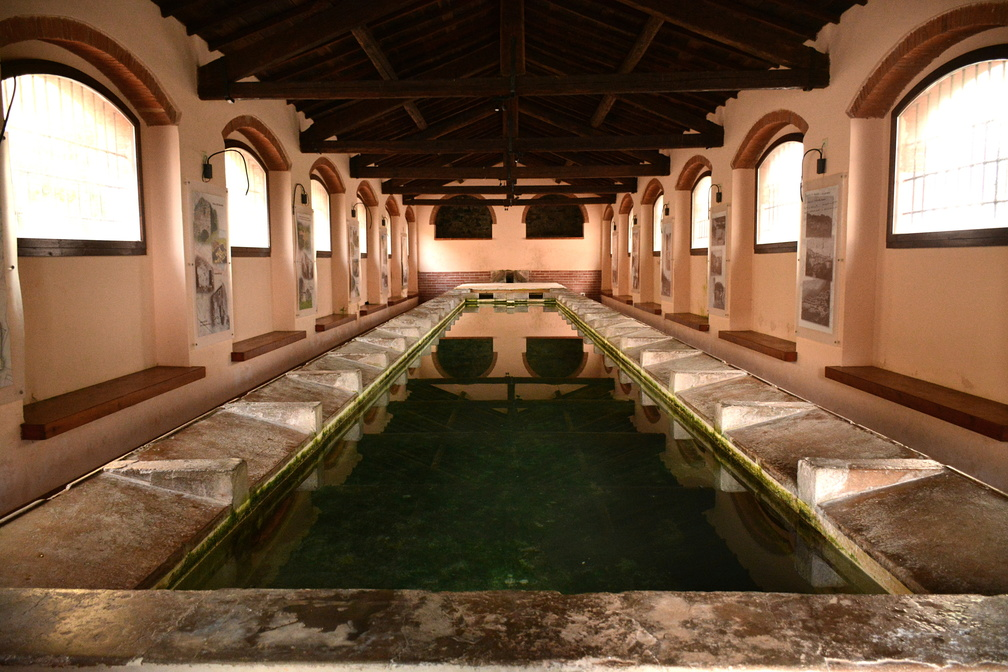
\includegraphics[width=7truecm]{slike/04_OdbojFoto.jpg}\hfill
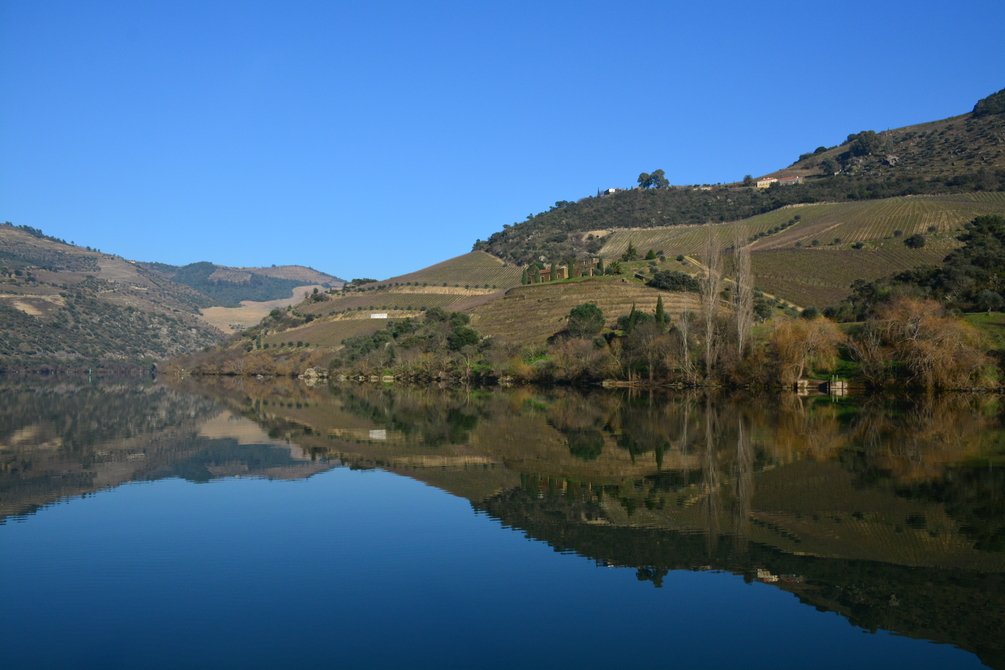
\includegraphics[width=7truecm]{slike/04_Douro.jpeg}
\caption{Odboj na vodni gladini. Pri majhnih vpadnih kotih je odbojnost
majhna, zato vidimo dno korita, pri večjih
vpadnih kotih postane odbojnost tako velika, da vidimo samo še odboj (levo).
Mirna rečna gladina pri velikih vpadnih kotih deluje kot zrcalo (desno).}
\label{fig:04_OdbojFoto}
\end{figure}

Poglejmo še primer transverzalne magnetne polarizacije. Narišemo odvisnost
amplitudne odbojnosti $r$ in amplitudne prepustnosti $t$ od vpadnega kota 
(slika~\ref{fig:04_redtm}\,a). Zaradi začetne izbire smeri odbite jakosti
električnega polja je predznak pri pravokotnem vpadu drugačen kot pri 
polarizaciji TE in je pozitiven, čeprav se faza valovanja obrne. 
Z naraščajočim vpadnim kotom se amplitudna
odbojnost zmanjšuje in doseže vrednost $r=-1$, ko se vpadni kot
približuje $\alpha = 90\si{\degree}$. 

Vidimo, da pri nekem kotu zavzame  
vrednost $r = 0$. Vpadni kot, pri katerem je odbojnost za TM polarizirano
valovanje enaka nič, imenujemo Brewstrov kot $\alpha_B$ po škotskem 
znanstveniku Siru Davidu Brewstru (1781--1868). Ta pojav ima pomembno in uporabno
posledico, da je celotno TM polarizirano valovanje pri Brewstrovem kotu prepuščeno. 
Ker amplitudna odbojnost pri Brewstrovem kotu zamenja predznak, se pri tem
kotu tudi spremeni faza odbite svetlobe: pri kotih $\alpha < \alpha_B$ se valovanje
odbije z nasprotno fazo, pri kotih $\alpha > \alpha_B$ pa se TM polarizirano
valovanje odbije z isto fazo.
\begin{figure}[ht]
\centering
\def\svgwidth{140truemm} 
\input{slike/04_redtm.pdf_tex}
\caption{Odvisnost amplitudne odbojnosti in amplitudne prepustnosti (a) ter odbojnosti in 
prepustnosti (b) za TM polarizirano valovanje v odvisnosti od vpadnega kota $\alpha$. Kot
$\alpha_B$ označuje Brewstrow kot.}
\label{fig:04_redtm}
\end{figure}

Odbojnost in prepustnost TM polariziranega valovanja sta prikazani na 
sliki~\ref{fig:04_redtm}\,b. Odbojnost od začetne vrednosti pri $\alpha=0$
pojema z naraščajočim vpadnim kotom do vrednosti 0, ki jo doseže pri 
Brewstrovem vpadnem kotu $\alpha_B$. Nato odbojnost strmo naraste z naraščajočim vpadnim
kotom do vrednosti 1. Pri velikih vpadnih kotih je zato
gladka meja z optično gostejšo snovjo videti kot zrcalo. Prepustnost preprosto izračunamo 
kot $\mathcal{T} = 1- \mathcal{R}$.

\subsection*{Brewstrov kot}
Brewstrov kot smo vpeljali kot vpadni kot, pri katerem je odbojnost
TM polariziranega valovanja enaka nič. Poglejmo, pri katerem
vpadnem kotu se to zgodi. Amplitudna odbojnost $r$ je po enačbi~(\ref{eq:04_40})
enaka:
\beq
r = \frac{\tan(\alpha-\beta)}{\tan(\alpha+\beta)}.
\label{eq:04_50}
\eeq
Pri vrednosti $\alpha + \beta = \pi/2$ imenovalec v izrazu za $r$ 
naraste v neskončnost. Ker je števec vedno različen od nič -- saj
sta po lomnem zakonu vpadni in lomni kot vedno različna -- je pri 
vrednosti $\alpha + \beta = \pi/2$ odbojnost enaka nič.
Izračunamo $\sin \beta = \sin (\pi/2-\alpha) = \cos \alpha$. 
Iz lomnega zakona (enačba~\ref{eq:04_18}) sledi:
\beq
n_1 \sin \alpha= n_2 \sin \beta= n_2 \cos \alpha.
\label{eq:04_51}
\eeq
Za Brewstrov kot tako velja:
\boxeq{eq:Brewstrovkot}{
\tan \alpha_B = \frac{n_2}{n_1}.
}
Pri prehodu iz zraka v steklo je $\alpha_B = 56\si{\degree}$ in na prehodu
iz zraka v vodo $\alpha_B = 53\si{\degree}$. 

Še enkrat povzemimo pomen Brewstrovega kota: odbojnost za TM polarizirano
valovanje je enaka nič, prepustnost za TM polarizirano valovanje pa enaka 1. Če 
torej TM polarizirana svetloba vpada na mejo pod Brewstrovim kotom, je vsa svetloba
prepuščena. Kadar pa osvetljujemo mejno ploskev z nepolarizirano svetlobo, se 
pri kotu $\alpha_B$ od mejne ploskve odbije samo TE polarizirano
valovanje, TM pa je v celoti prepuščeno. Na ta preprost način
iz nepolarizirane svetlobe dobimo linearno polarizirano valovanje.
\vglue-5truemm
\begin{remark}
Pri Brewstrovem kotu je odbojnost TM polariziranega valovanja točno 
enaka nič, vendar je tudi pri kotih, ki so blizu $\alpha_B$, 
odbojnost precej manjša kot za TE polarizirano valovanje. 
To s pridom uporabljamo pri polarizacijskih sončnih očalih ali fotografskih
filtrih. Ker se od površine, na primer vodne gladine, zasnežene pokrajine
ali gladke ceste, odbije razmeroma malo TM polariziranega valovanja, 
je odbita svetloba pretežno TE linearno polarizirana. Če sončna
očala ali fotografski filter delujejo kot polarizator, ki TE polarizirane 
svetlobe ne prepušča, bistveno zmanjšamo količino odbite svetlobe in 
``bleščanje'' površine. Sončna očala so linearni polarizatorji, večina 
fotografskih polarizacijskih filtrov pa je cirkularnih polarizatorjev,
saj bi vstopna linearna polarizacija motila delovanje svetlomera.
\begin{figure}[ht]
\centering
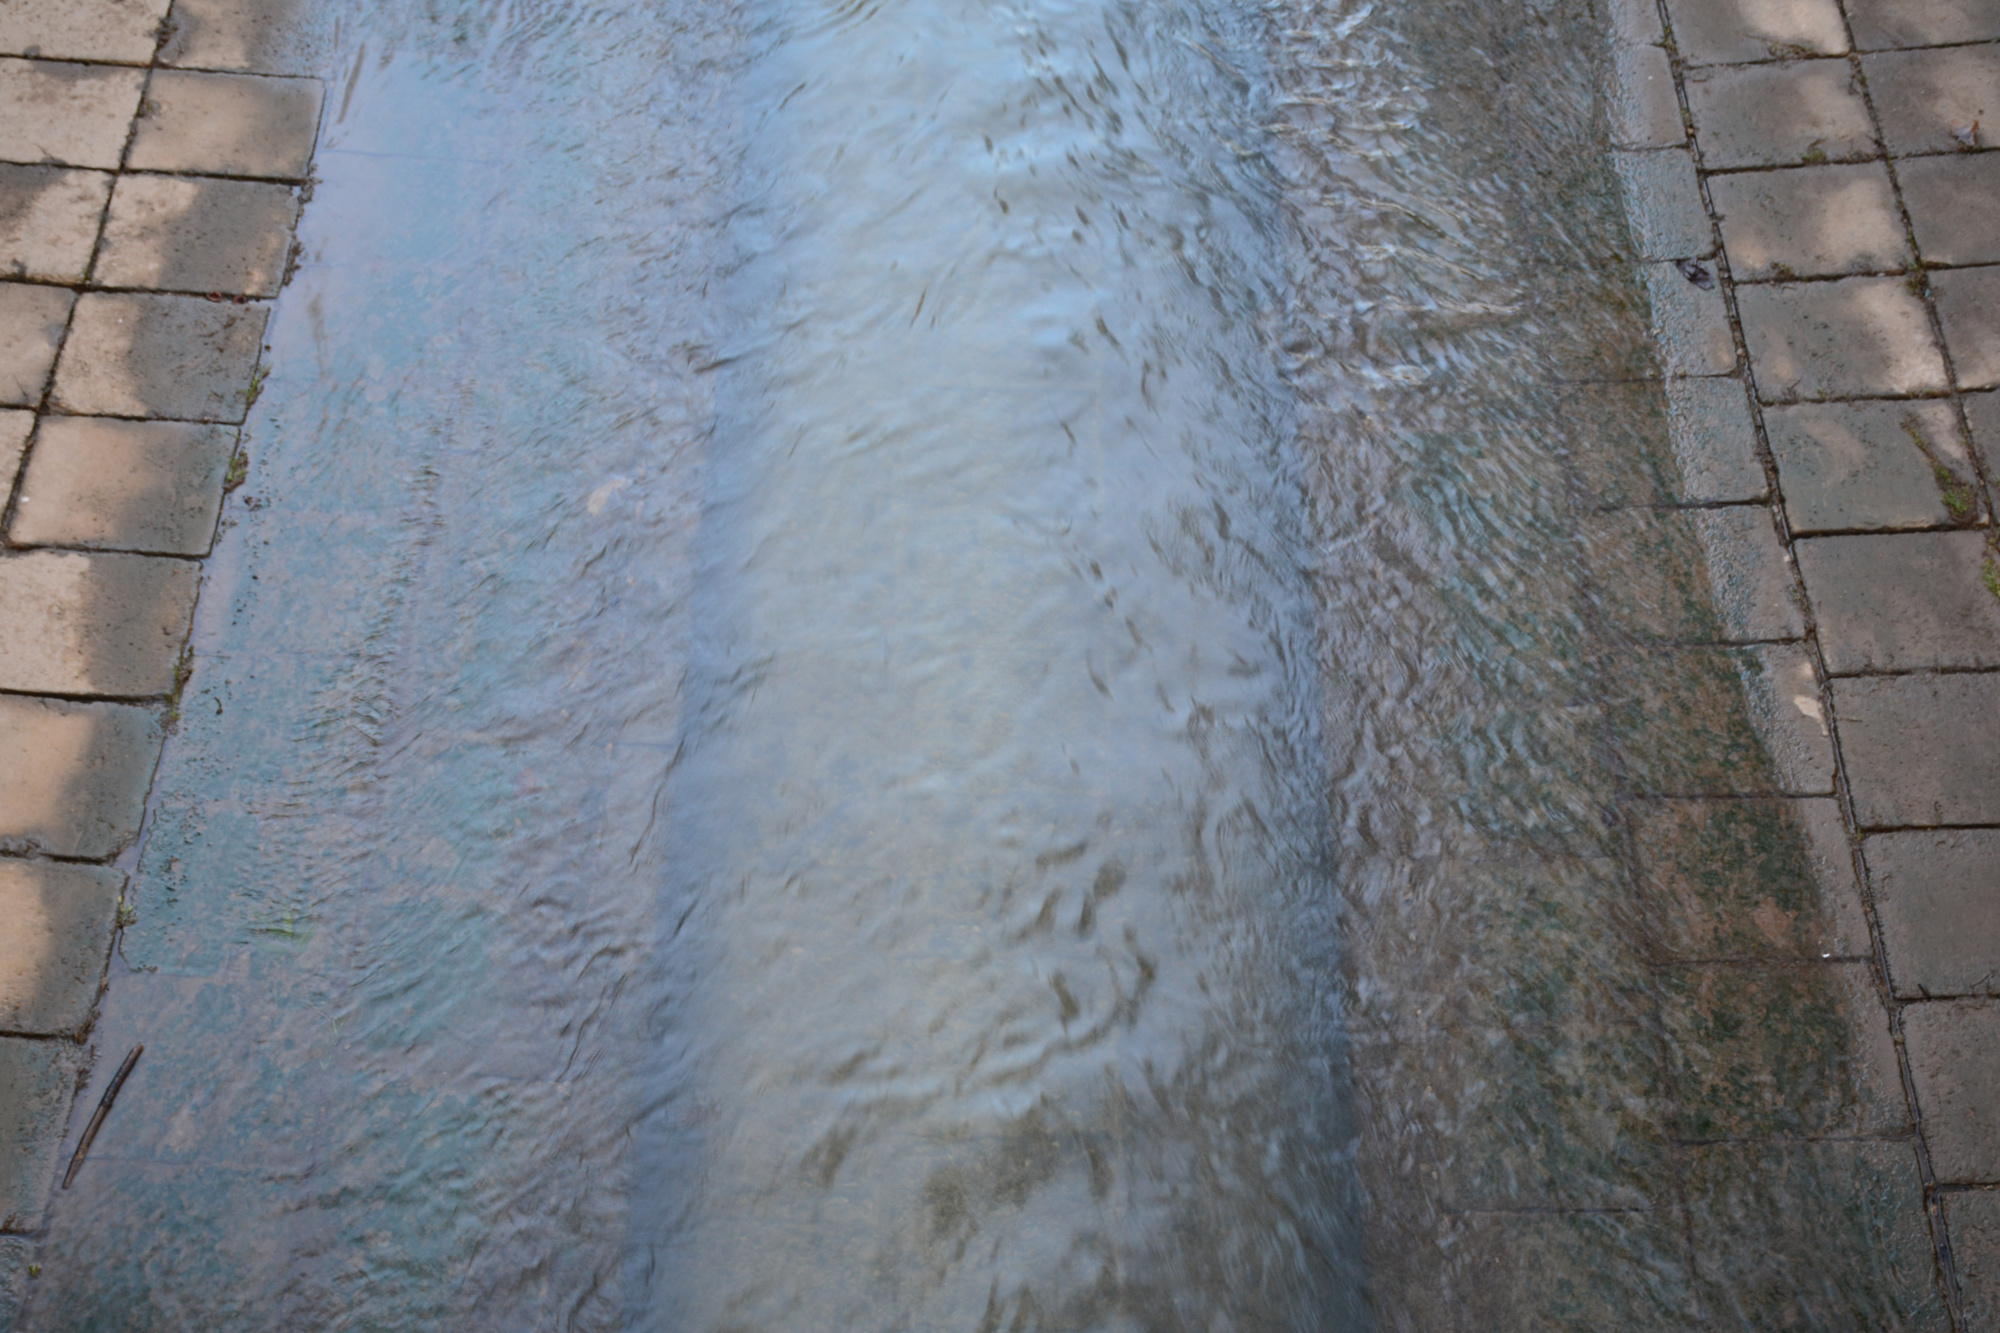
\includegraphics[width=7truecm]{slike/04_photos_voda1.jpg}\hfill
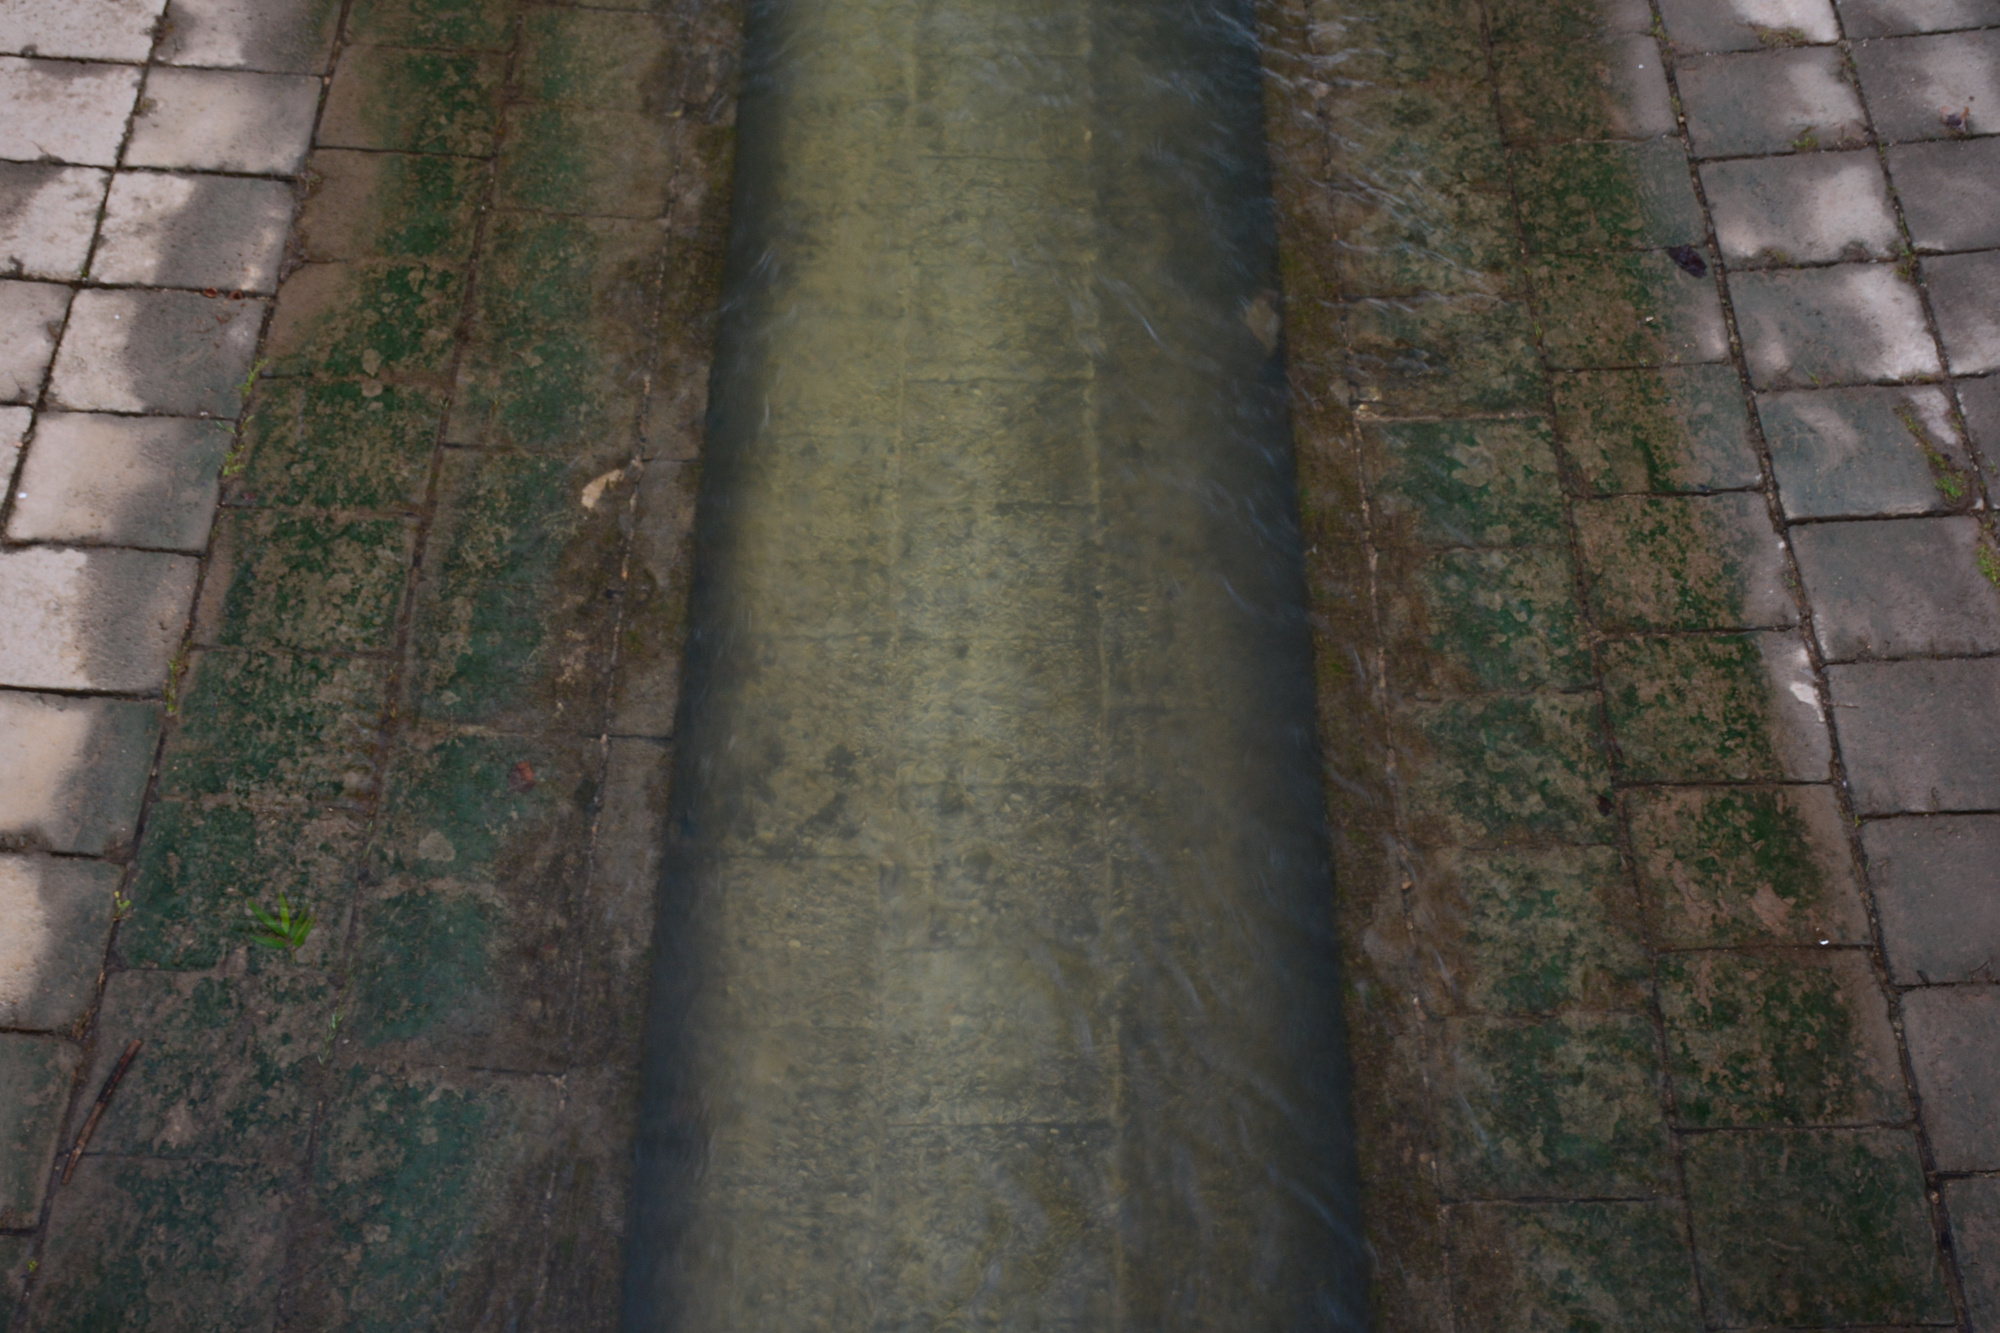
\includegraphics[width=7truecm]{slike/04_photos_voda2.jpg}
\caption{Odsev na vodni gladini preprečuje, da bi videli v globino vode (levo).
Ker je odbita svetloba pretežno linearno polarizirana, jo s polarizacijskim 
filtrom lahko zaustavimo in tako vidimo dno potoka (desno).}
\label{fig:04_odsevvoda}
\end{figure}

\begin{figure}[ht]
\centering
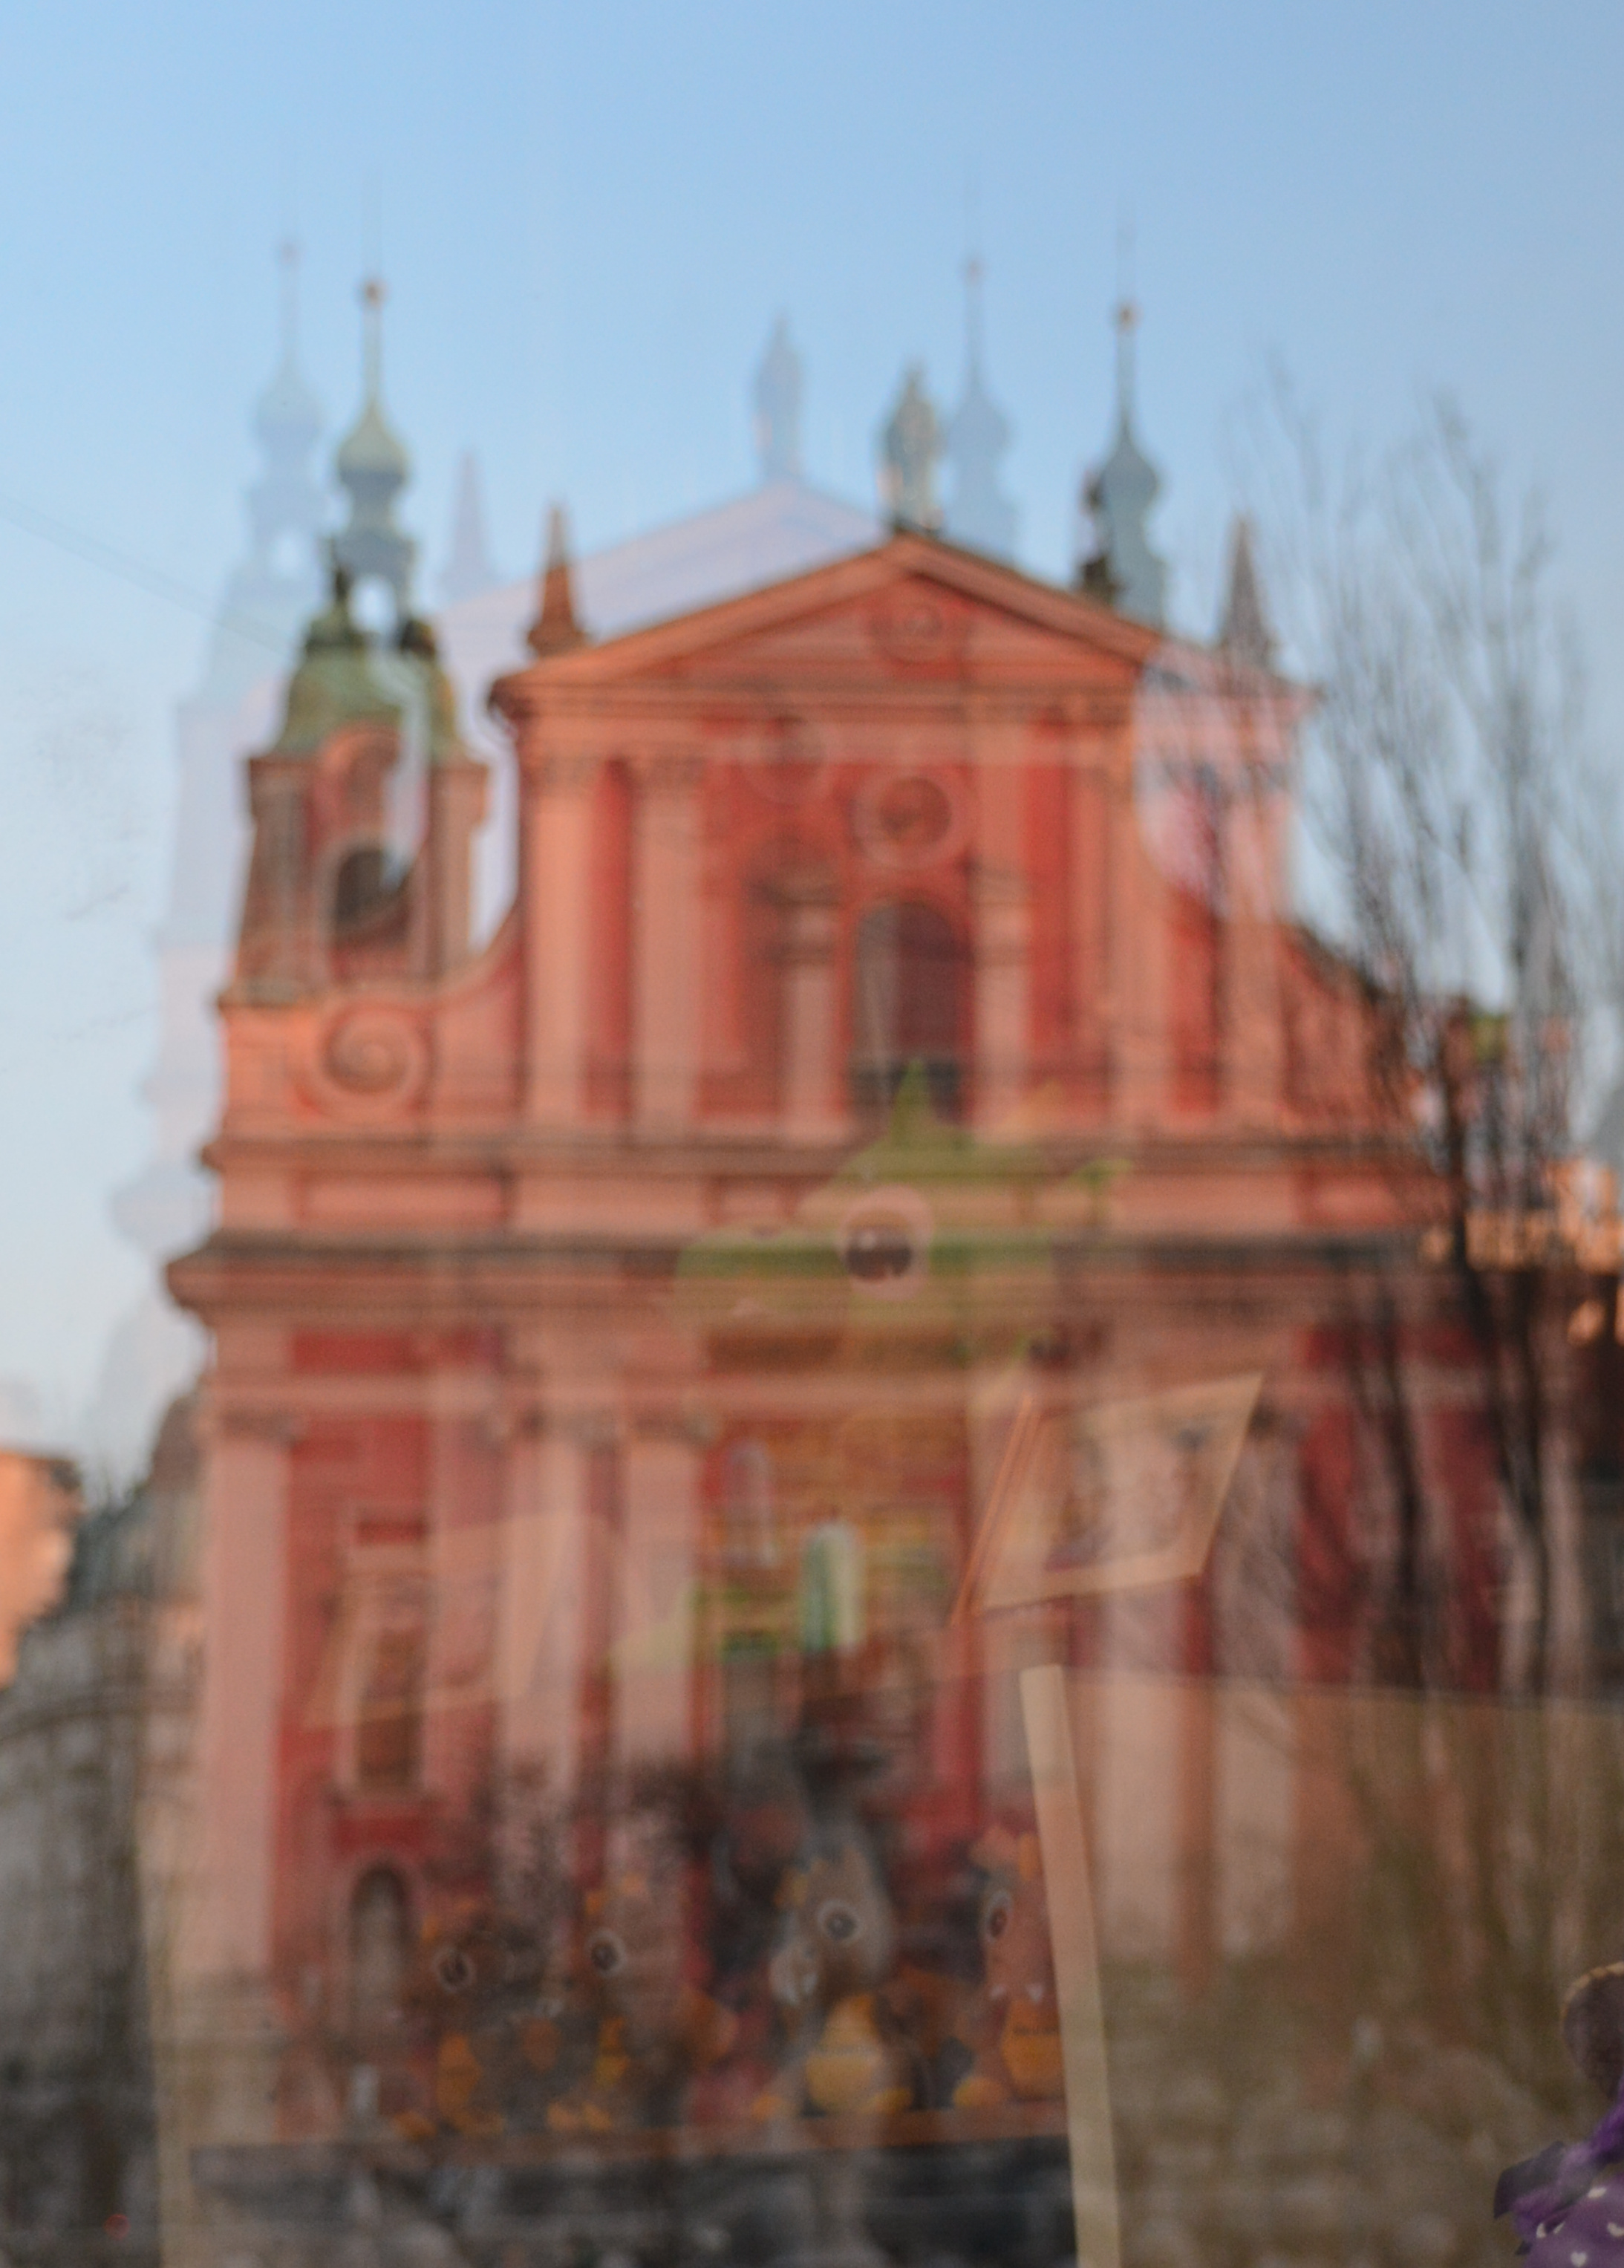
\includegraphics[width=6truecm]{slike/04_photos_zmaj2.jpg}\qquad \qquad

\includegraphics[width=6truecm]{slike/04_photos_zmaj1.jpg}
\caption{Odsev v izložbenem oknu (levo) in isti motiv, slikan s polarizacijskim 
filtrom (desno), ki omogoča pogled v izložbo.}
\label{fig:04_odsevzmaj}
\end{figure}
\begin{figure}[!h]
\centering
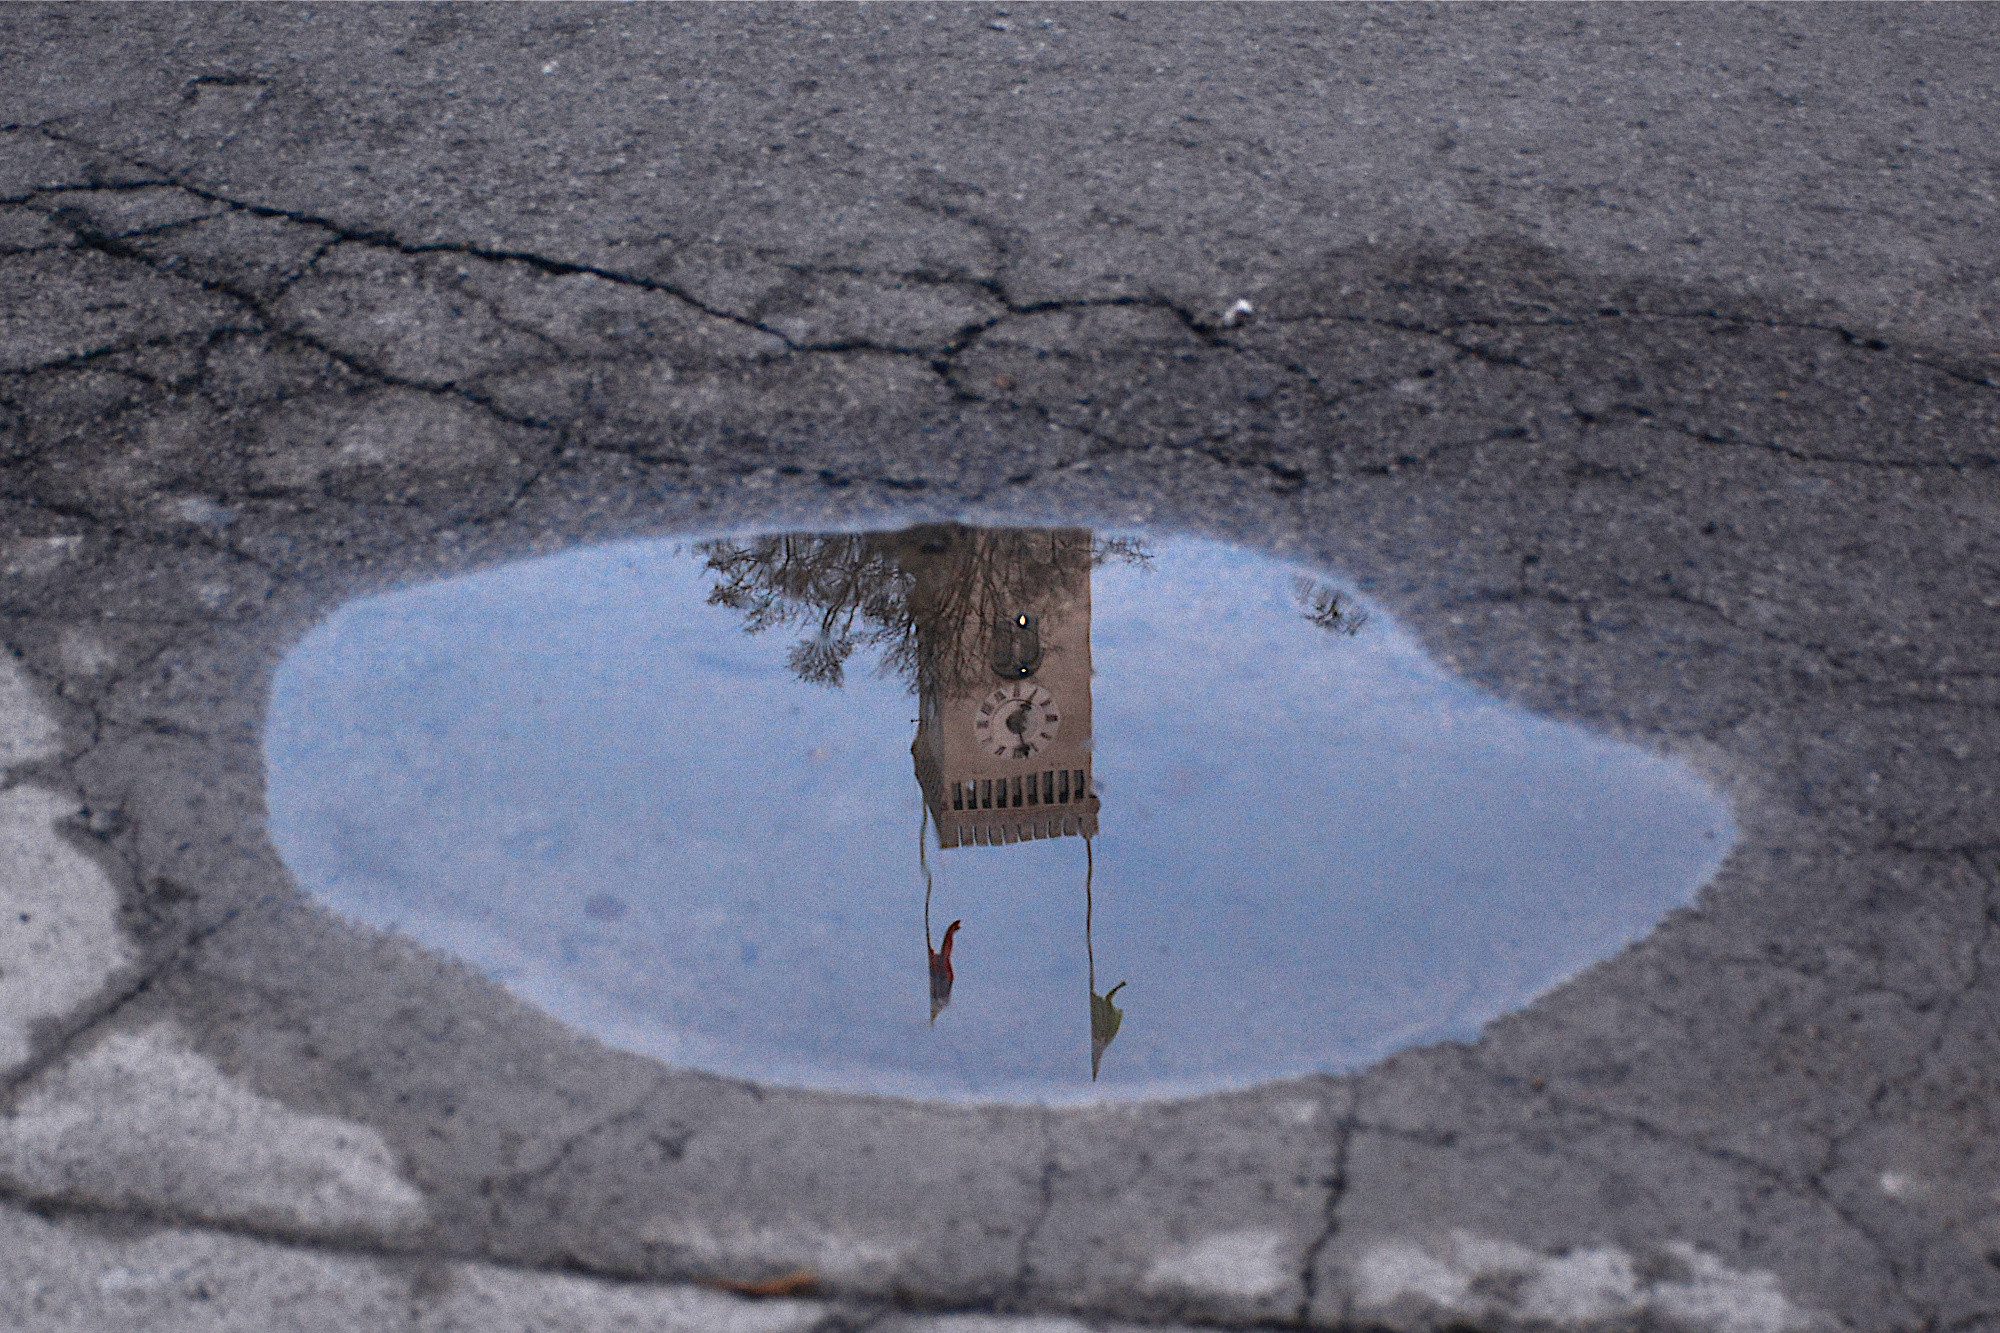
\includegraphics[width=7truecm]{slike/04_photos_grad1.jpg}\hfill
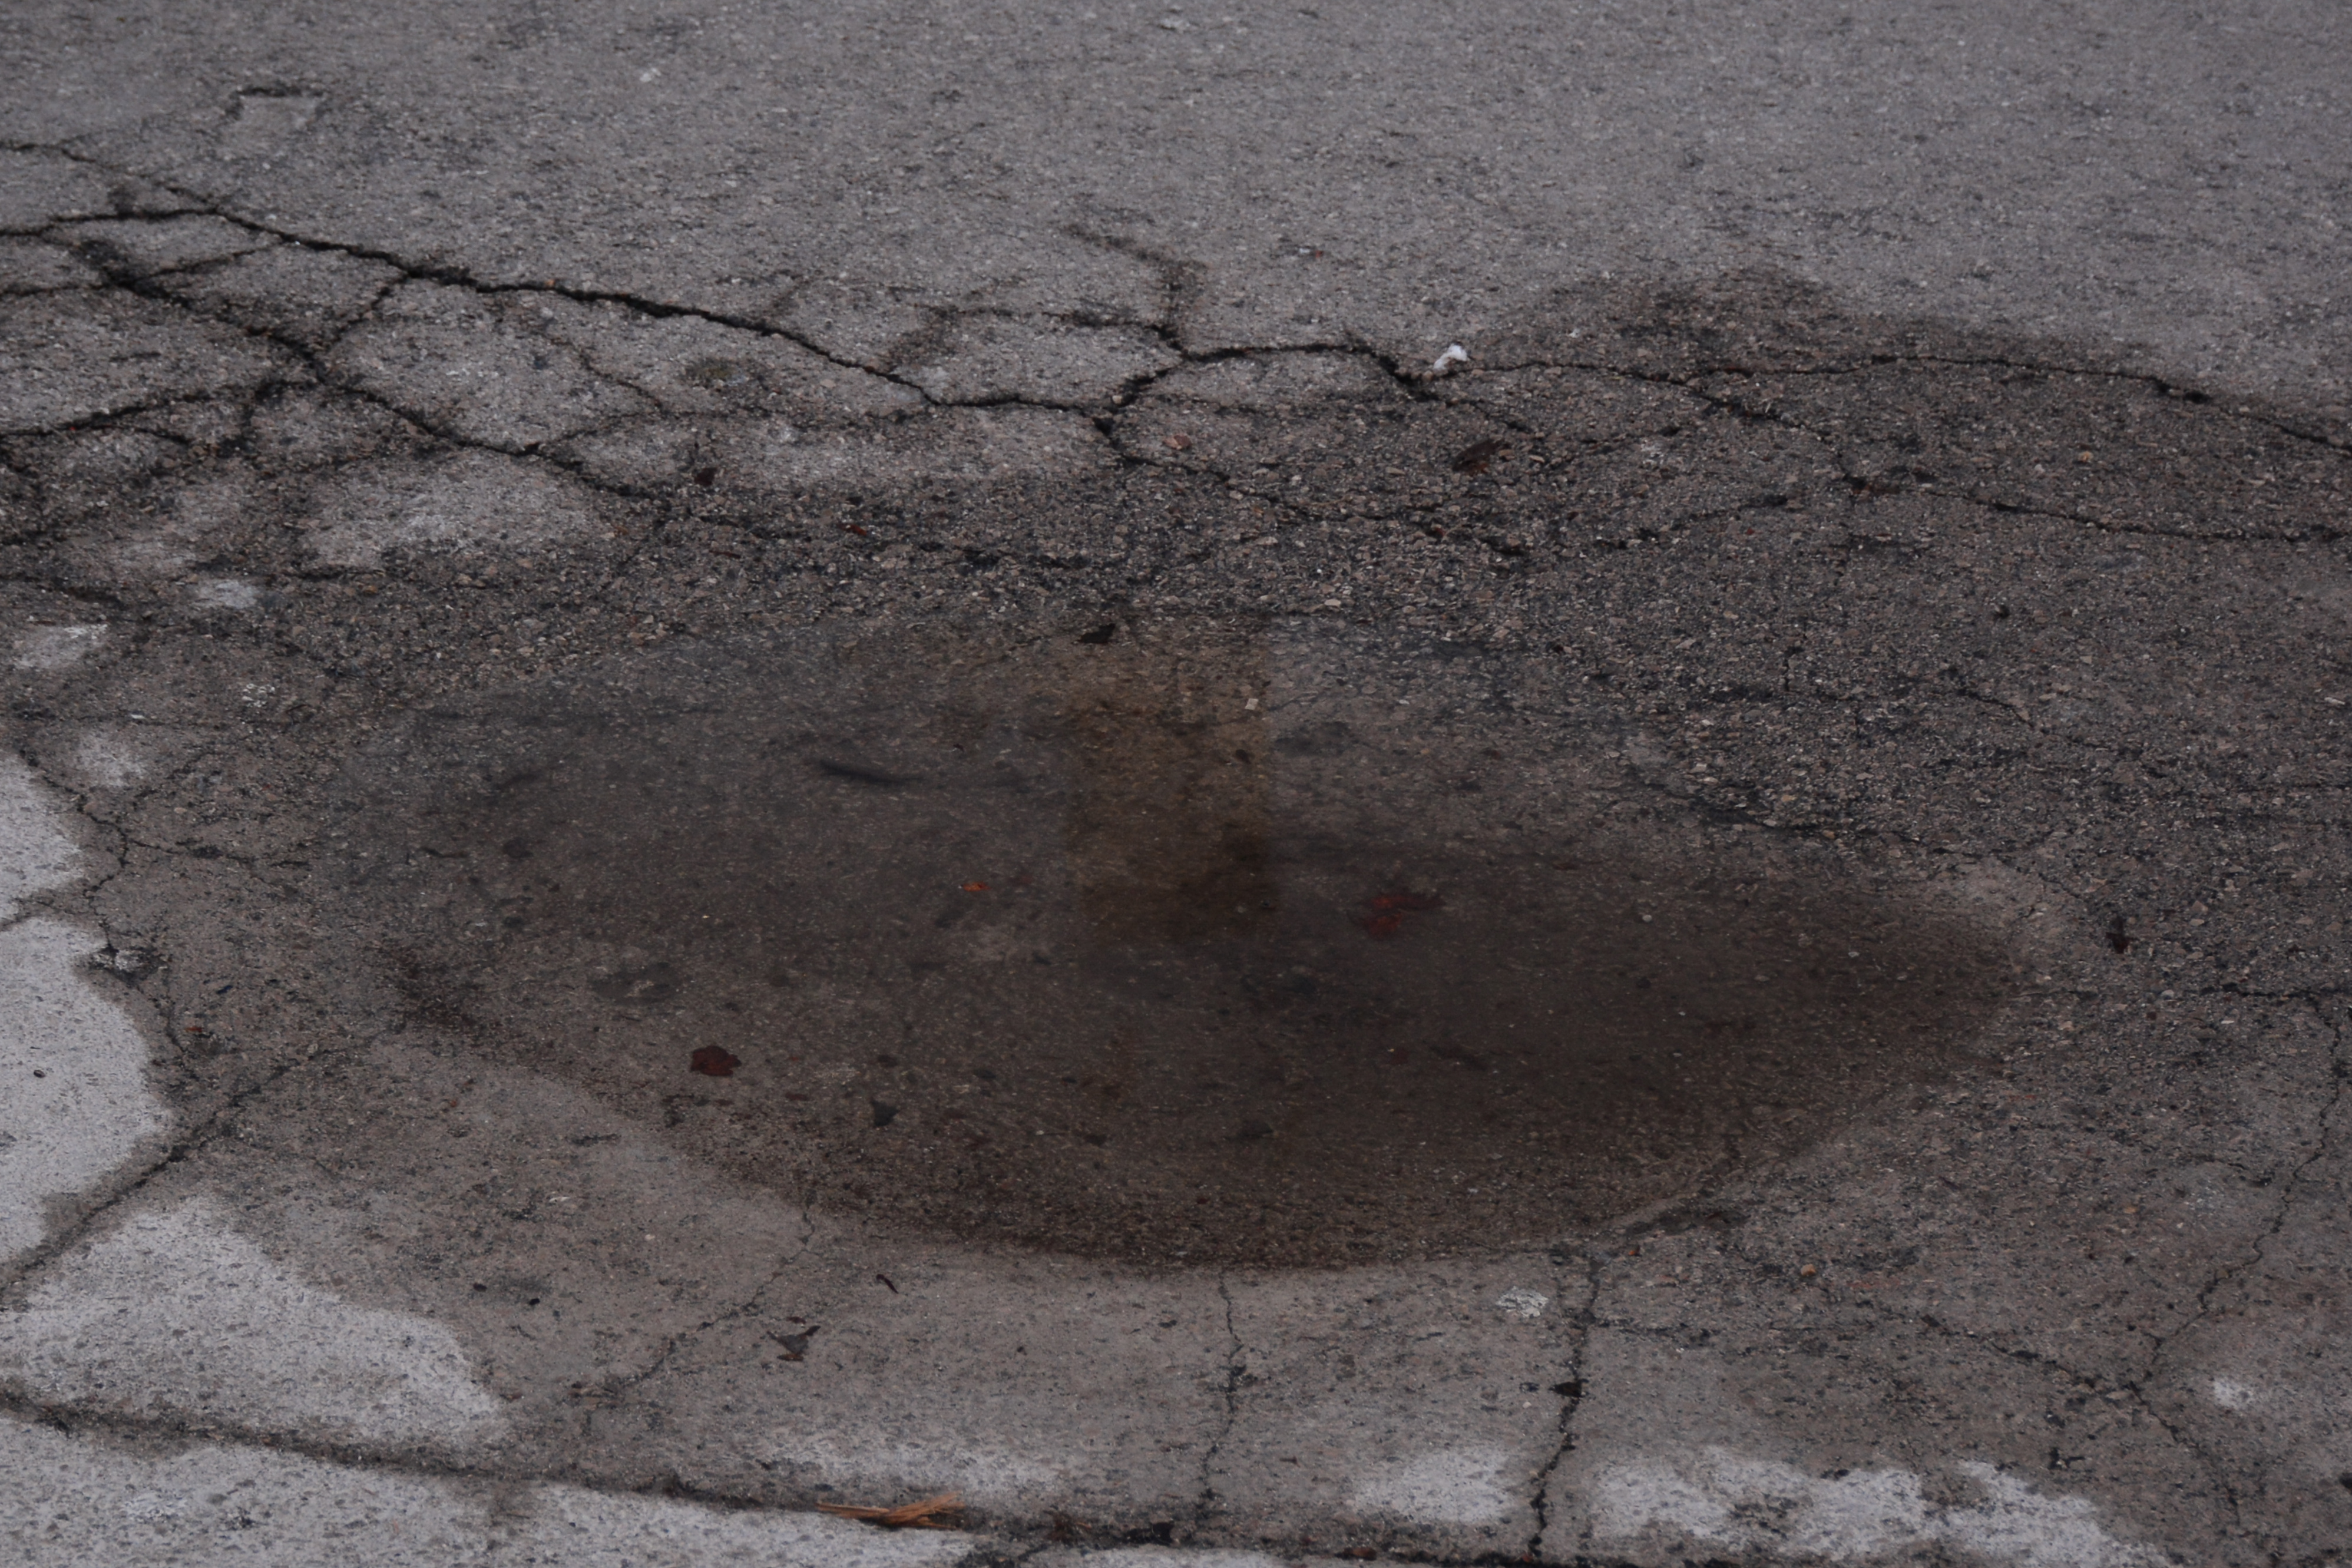
\includegraphics[width=7truecm]{slike/04_photos_grad2.jpg}
\caption{Odsev v luži (levo) in isti motiv, slikan s polarizacijskim filtrom (desno). 
Polarizirano odbito svetlobo zaustavi fotografski filter, zato odsev ni več viden,
vidno pa je dno luže.}
\label{fig:04_odsevgrad}
\end{figure}
\begin{figure}[!h]
\centering
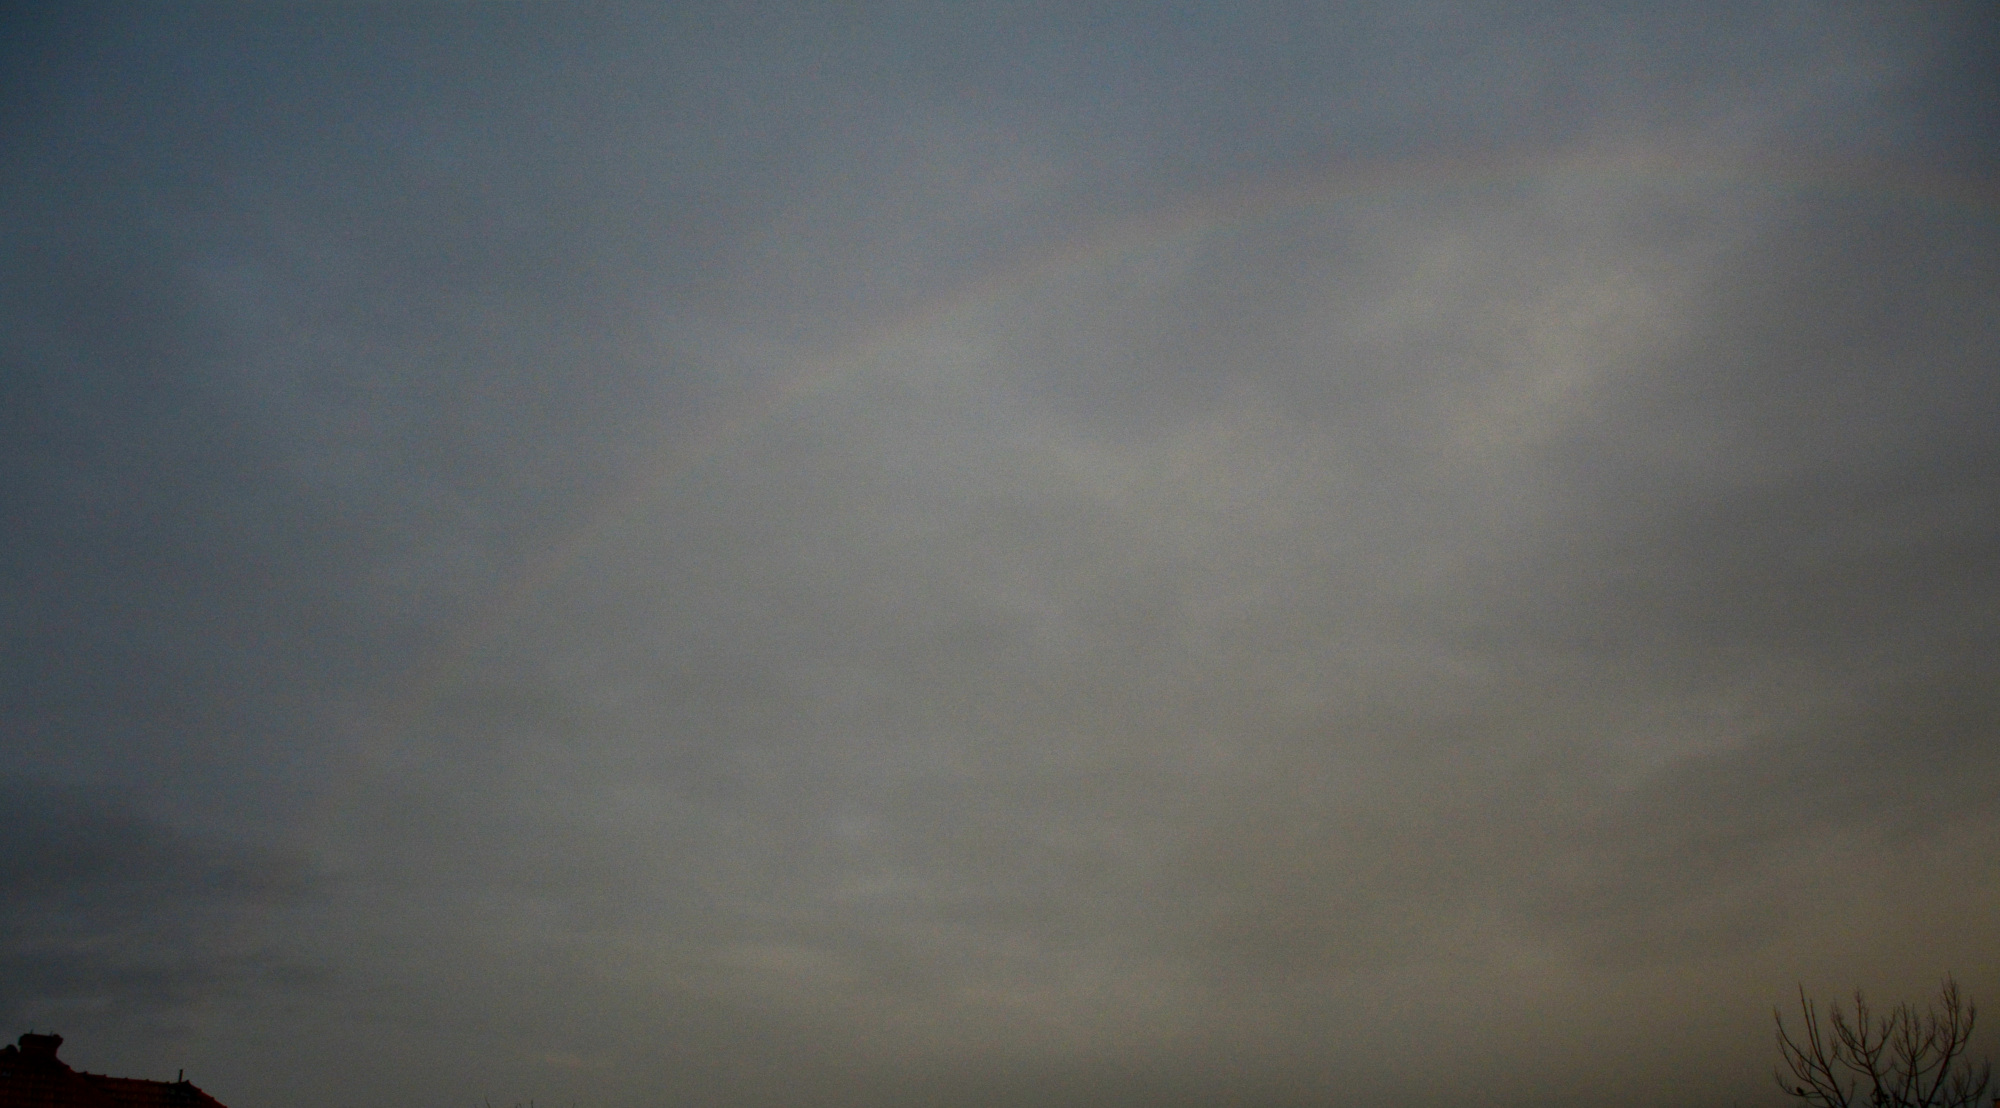
\includegraphics[width=7truecm]{slike/04_PolMavrica_a.jpg}\hfill
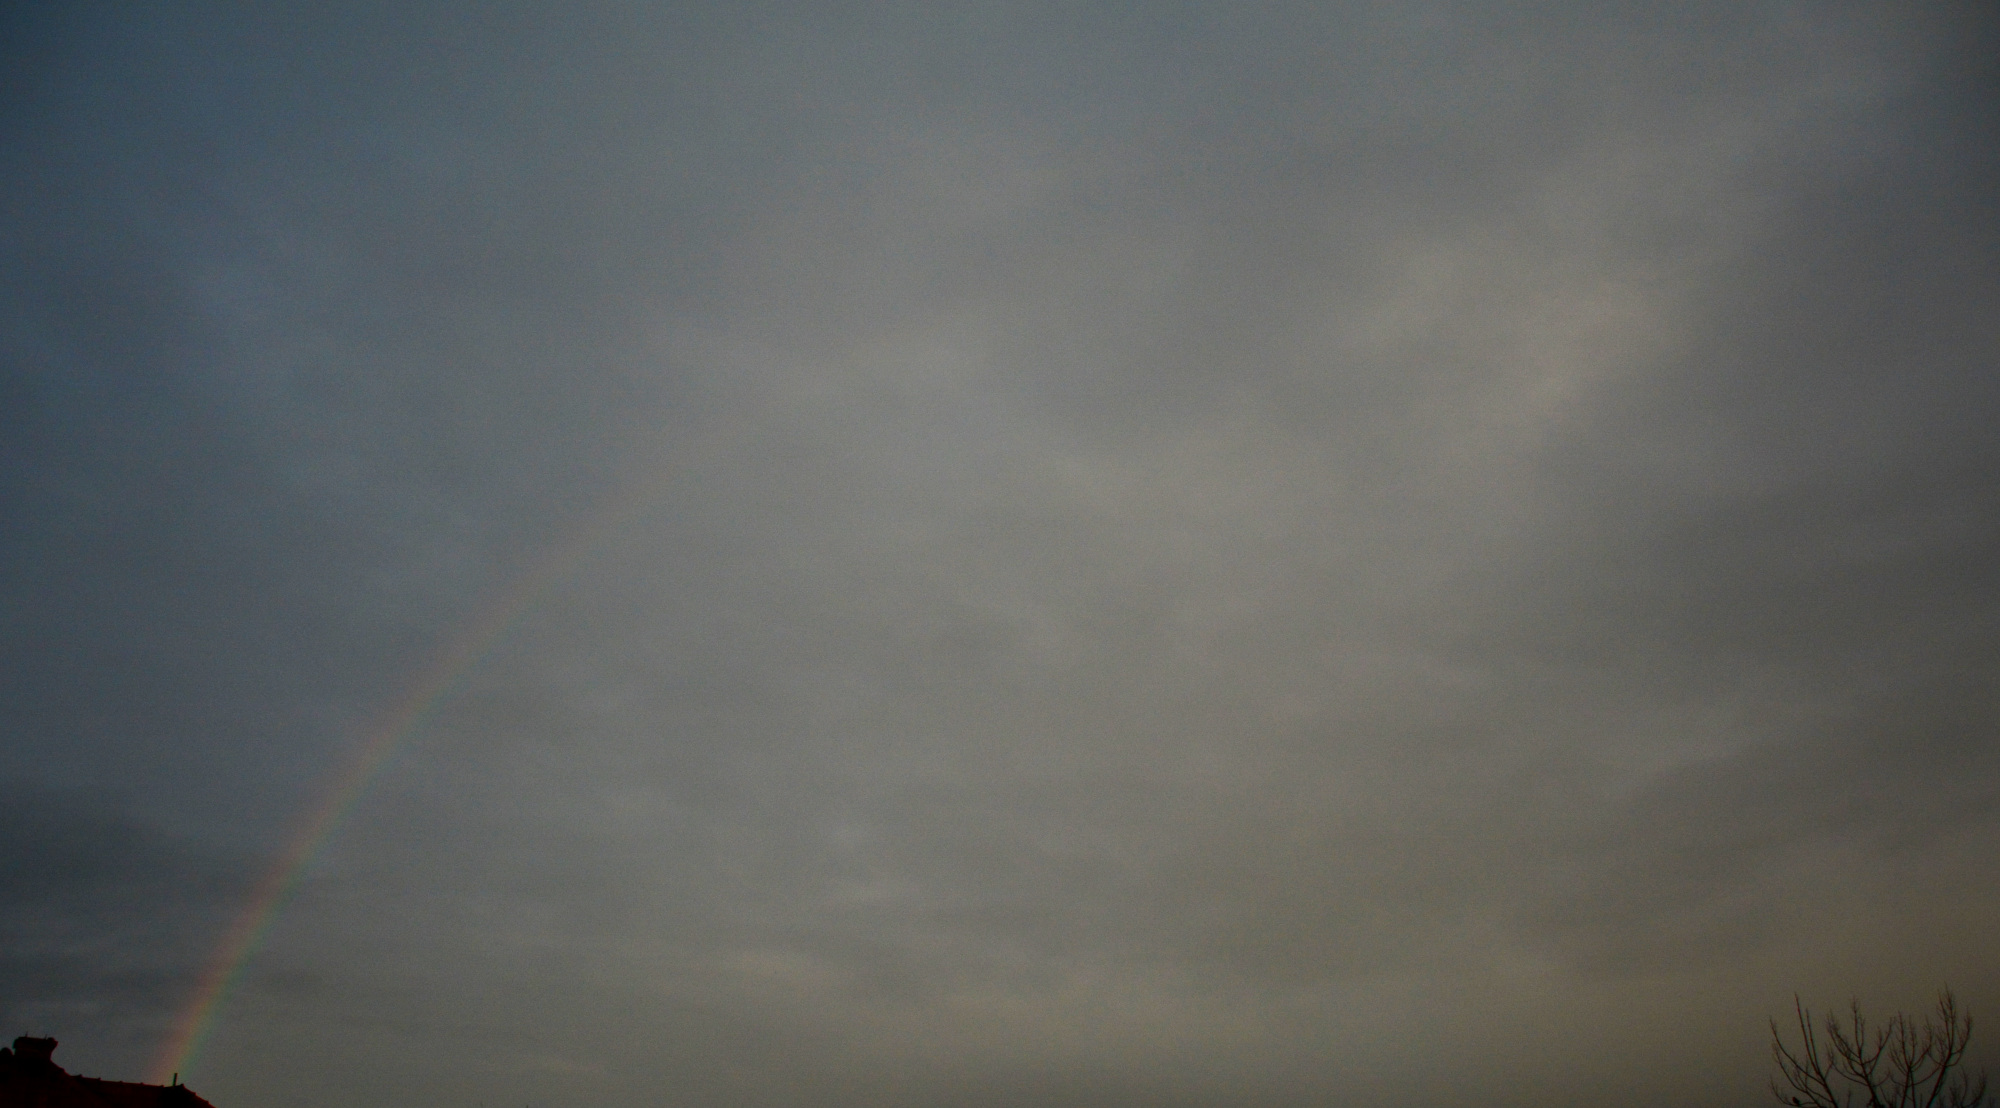
\includegraphics[width=7truecm]{slike/04_PolMavrica_b.jpg}
\caption{Mavrica nastane z odbojem svetlobe v dežnih kapljicah (glej poglavje~\ref{chap:disperzija}).
Ker je odbojni kot blizu Brewsterjevega kota, je mavrica pretežno polarizirana, kar pokažemo z linearnim 
polarizatorjem (smer polarizatorja označuje puščica). Šibko vidni zgornji lok mavrice na desni sliki povsem 
izgine, osnovni mavrični lok pa je viden le še ob robovih.}
\label{fig:04_MavricaFoto}
\end{figure}
\end{remark}

\section{Prehod v optično redkejšo snov in totalni odboj}
Pri prehodu v snov z manjšim lomnim količnikom pride do novih zanimivih pojavov.
Primer tega je prehod svetlobe iz vode ali stekla v zrak, ko je $n_1>n_2$.
Izhajamo iz lomnega zakona (enačba~\ref{eq:04_18}) in zapišemo lomni kot:
\beq
\beta = \arcsin \left(\frac{n_1}{n_2}\sin \alpha\right)\!\!.
\label{eq:04_52}
\eeq
Pri določeni vrednosti vpadnega kota $\alpha_m$ 
argument doseže vrednost $1$ in lomni kot
postane enak $\beta = 90\si{\degree}$. Za vpadne kote, ki so večji od 
mejnega in za katere velja
$\alpha> \alpha_m$, enačba nima več rešitve. Takrat govorimo o totalnem 
ali popolnem odboju. Mejni kot totalnega odboja izračunamo kot:
\boxeq{eq:totalni}{
\alpha_m = \arcsin\left(\frac{n_2}{n_1}\right)\!\!.
}
V steklu z lomnim količnikom $n_1=1,5$ je mejni kot totalnega odboja
enak $\alpha_m = 41,8\si{\degree}$, v vodi z lomnim količnikom 
$n_1 = 1,33$ pa $\alpha_m = 48,7\si{\degree}$.
\begin{figure}[ht]
\centering
\def\svgwidth{140truemm} 
\input{slike/04_totalni.pdf_tex}
\caption{Svetloba vpada iz snovi z večjim lomnim količnikom v snov z manjšim lomnim količnikom.
Pri vpadnih kotih, ki so večji od mejnega kota totalnega odboja $\alpha_m$, se svetloba totalno odbije (a). Pri računu
si pomagamo s sliko loma (b).}
\label{fig:04_totalni}
\end{figure}

Izračunajmo odbojnost in prepustnost najprej za TE polarizacijo.
Po enačbi~(\ref{eq:TEr}) je:
\beq
r = \frac{n_1 \cos \alpha - n_2 \sqrt{1 - (\sin \alpha \cdot n_1/n_2)^2}}
{n_1 \cos \alpha + n_2 \sqrt{1 - (\sin \alpha \cdot n_1/n_2)^2}}.
\label{eq:04_53}
\eeq
Za vrednosti vpadnega kota $\alpha > \alpha_m$ je argument korena
negativen, zato postane člen imaginaren. Zapišimo:
\beq
r = \frac{n_1 \cos \alpha - i n_2 \kappa}{n_1 \cos \alpha + i n_2\kappa},
\label{eq:04_54}
\eeq
pri čemer je:
\beq
\kappa = \sqrt{\left(\frac{n_1}{n_2}\sin \alpha \right)^2-1}  = 
\sqrt{\left(\frac{\sin \alpha}{\sin \alpha_m}\right)^2 -1}.
\label{eq:04_55}
\eeq
Potem izračunamo odbojnost $\mathcal{R}$:
\beq
\mathcal{R} = |r|^2 = \frac{n_1 \cos \alpha -i n_2\kappa}{n_1 \cos \alpha +i n_2\kappa}
\cdot \frac{n_1 \cos \alpha +i n_2\kappa}{n_1 \cos \alpha -i n_2\kappa} = 1.
\label{eq:04_56}
\eeq
Pri vpadnih kotih, ki so večji od mejnega kota totalnega odboja, je $\mathcal{R} = 1$
in vsa vpadna svetloba se odbije. Za smer odbitega žarka velja odbojni zakon. 
\begin{figure}[ht]
\centering
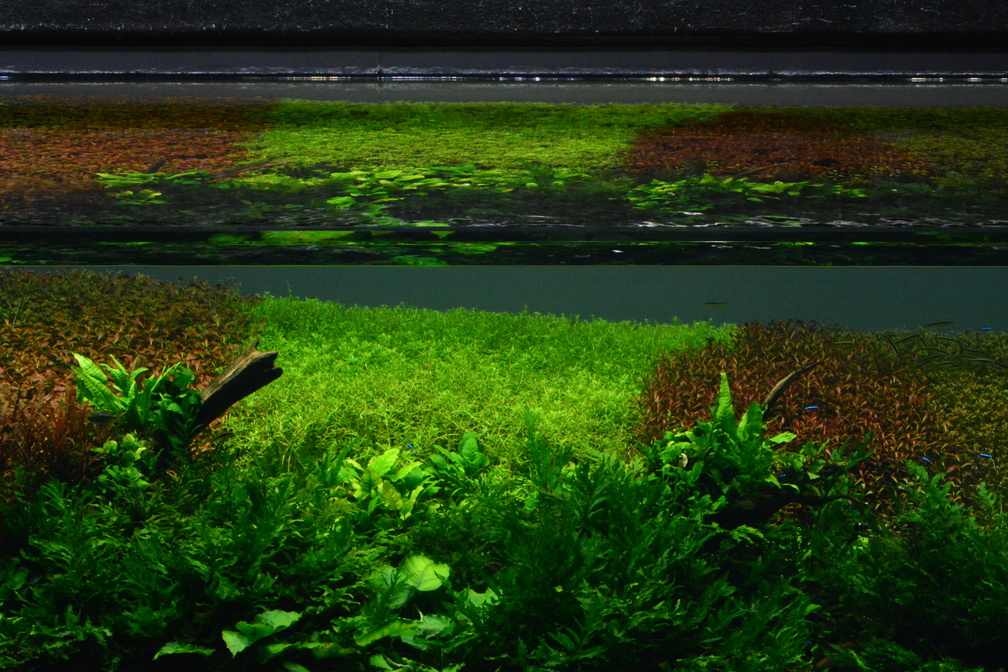
\includegraphics[width=10truecm]{slike/04_TotalniOdbojFoto.jpg}
\caption{Totalni odboj na gladini akvarija}
\vglue-5truemm
\label{fig:04_TotalniFoto}
\end{figure}

Narišimo amplitudno odbojnost in amplitudno prepustnost za TE valovanje 
(slika~\ref{fig:04_goste}\,a). 
Ker je $n_1>n_2$, je amplitudna odbojnost pri pravokotnem vpadu pozitivna. 
Pri pravokotnem vpadu svetlobe na optično redkejšo snov se torej
faza ohranja. Amplitudna odbojnost z naraščajočim vpadnim kotom narašča 
do vrednosti $r=1$, ki jo doseže pri mejnem kotu totalnega odboja. 
Prepustnost, ki jo izračunamo
kot $t = 1+r$, zavzame pri pravokotnem vpadu vrednost nekaj nad 1,
nato pa narašča do vrednosti $t=2$, ki jo doseže pri $\alpha = \alpha_m$. 
To, da je prepustnost večja od 1, nas ne sme motiti, saj gre za
razmerje med amplitudami valovanja in ne med energijskimi tokovi.
\begin{figure}[ht]
\centering
\def\svgwidth{140truemm} 
\input{slike/04_goste.pdf_tex}
\caption{Odvisnost amplitudne odbojnosti in amplitudne prepustnosti (a) ter odbojnosti in 
prepustnosti (b) za TE polarizirano valovanje v odvisnosti od vpadnega kota $\alpha$. 
Pri kotih, ki so večji od mejnega kota $\alpha_m$, se svetloba totalno odbije.}
\label{fig:04_goste}
\end{figure}

Na sliki (slika~\ref{fig:04_goste}\,b) sta prikazani še odbojnost $\mathcal{R}$ 
in prepustnost $\mathcal{T}$. Odbojnost od neke začetne vrednosti homogeno
narašča do $1$ pri mejnem kotu totalnega odboja. Za vse vpadne kote $\alpha$, ki
so večji od mejnega kota totalnega odboja $\alpha_m$, je odbojnost $\mathcal{R} = 1$ in 
prepustnost $\mathcal{T} = 0$.

Za TM polarizacijo amplitudna odbojnost, ki homogeno
narašča od začetne negativne vrednosti do 1 pri mejnem
kotu totalnega odboja, pri Brewstrovem kotu zavzame vrednost 0 (slika~\ref{fig:04_gostm}\,a). 
Tako sta pri prehodu TM polariziranega valovanja v optično redkejšo
snov pomembna dva kota: Brewstrov kot $\alpha_B$ in mejni kot totalnega odboja $\alpha_m$.
Pri prvem je odbojnost enaka nič, pri drugem pa 1. Amplitudna prepustnost $t$ pri mejnemu kotu 
totalnega odboja doseže vrednost $t>2$, 
saj v enačbi~(\ref{eq:TMt}) nastopa še razmerje lomnih količnikov, ki je 
večje od 1. 
\begin{figure}[ht]
\centering
\def\svgwidth{140truemm} 
\input{slike/04_gostm.pdf_tex}
\caption{Odvisnost amplitudne odbojnosti in amplitudne prepustnosti (a) ter odbojnosti in 
prepustnosti (b) za TM polarizirano valovanje v odvisnosti od vpadnega kota $\alpha$. 
Pri kotih, ki so večji od mejnega kota $\alpha_m$, se svetloba totalno odbije. Kot $\alpha_m$
označuje Brewstrov kot.}
\label{fig:04_gostm}
\end{figure}

Odbojnost in prepustnost sta prikazani na sliki~\ref{fig:04_gostm}\,b. Po pričakovanju 
odbojnost z naraščajočim kotom pojema do vrednosti 0, ki jo zavzame pri Brewstrovem kotu, 
nato pa strmo naraste do vrednosti 1, ki jo doseže pri mejnem kotu totalnega odboja. Pri večjih
kotih je odbojnost enaka 1. Prepustnost je največja pri Brewstrovem kotu, nato pa strmo
pade do vrednosti 0 pri totalnem odboju.

\begin{remark}
Če z žarkom svetlobe posvetimo v tanko plast z lomnim količnikom večjim od 
lomnega količnika okolice, lahko svetlobo ``ujamemo''. Zaradi
zaporednih totalnih odbojev namreč svetlobni žarek ostaja ujet v tanki plasti in se 
širi praktično brez izgub. Tako lahko na preprost način razložimo delovanje optičnih vlaken, 
po katerih svetloba potuje na zelo dolge razdalje. Optična vlakna so nepogrešljiva
pri modernih telekomunikacijah.
\begin{figure}[ht]
\centering
\def\svgwidth{130truemm} 
\input{slike/04_vlakno.pdf_tex}
\caption{Shema optičnega vlakna z lomnim količnikom $n_1$, ki je večji od lomnega količnika
okolice. Pri dovolj velikih vpadnih kotih se žarek svetlobe na stenah totalno odbije in svetloba
praktično brez izgub potuje po vlaknu.}
\label{fig:04_vlakno}
\end{figure}

\begin{figure}[ht]
\centering
\includegraphics[width=13truecm]{slike/04_vlakno_model.jpg}
\caption{V akrilni valj se svetlobi žarek ujame s totalnim odbojem podobno kot se žarek
ujame v optično vlakno.}
\label{fig:04_vlaknomodel}
\end{figure}
\end{remark}

\begin{remark}
Lomni količnik diamanta je razmeroma velik (okoli 2,4), zato je mejni kot 
totalnega odboja razmeroma majhen ($\alpha_m \approx 25\si{\degree}$). Diamanti so praviloma
obrušeni tako, da se vpadna svetloba na spodnjih ploskvah totalno odbije, kar da diamantom značilen
lesk. Velik lomni količnik pomeni veliko območje vpadnih kotov svetlobe, pod katerim se 
diamant blešči, zato so diamanti še posebej priljubljeni za izdelavo nakita.
\vglue-0.3truecm
\begin{figure}[!h]
\centering
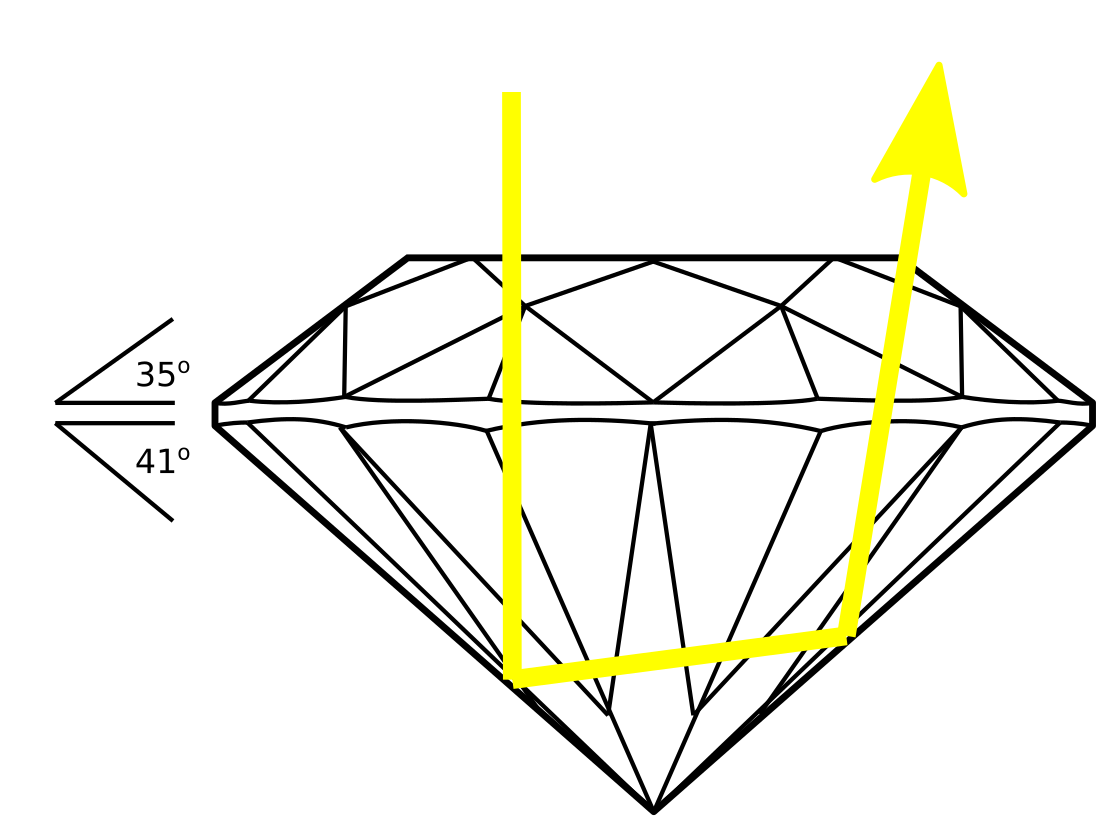
\includegraphics[height=3.7truecm]{slike/04_diamant.png}\qquad
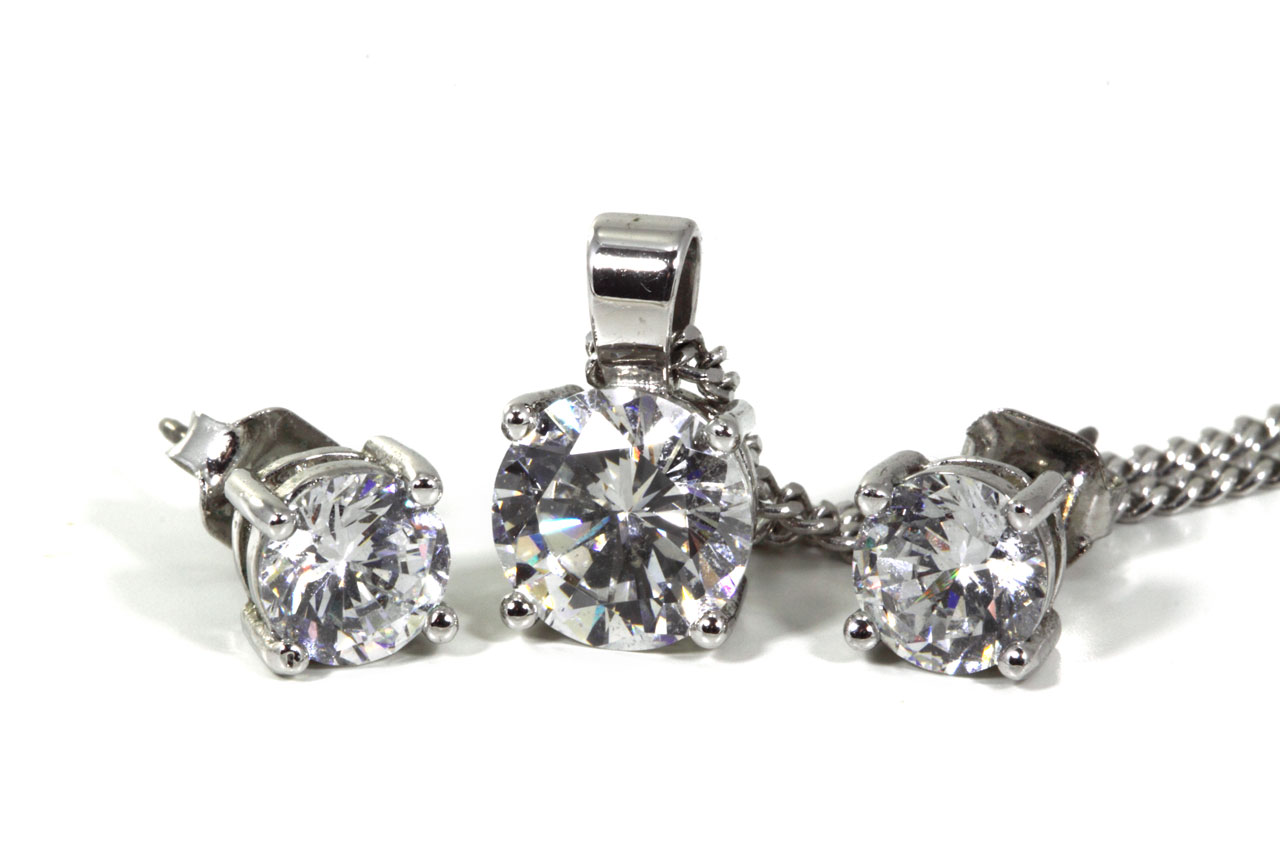
\includegraphics[height=3.7truecm]{slike/04_nakit.jpg}\hfill
\caption{Diamanti so brušeni tako, da se na spodnjih ploskvah vpadna svetloba totalno odbije (levo), 
kar jih naredi še posebej privlačne za nakit (Foto: Vera Kratochvil, PublicDomainPictures).}
\label{fig:04_diamanti}
\end{figure}
\end{remark}

\section{Evanescento polje}
Povedali smo, da se pri totalnem odboju vsa vpadna svetloba odbije. Izračunajmo
zdaj jakost električnega polja na obeh straneh meje med snovema.

Naj svetloba vpada na ravno mejo dveh neprevodnih, homogenih 
in izotropnih snovi, za kateri velja $n_1>n_2$. 
Amplitudni odbojnosti za obe polarizaciji zapišemo kot (enačbi~\ref{eq:04_54} in 
\ref{eq:TMr}):
\beq
r_{\mathrm{TE}} = \frac{n_1 \cos \alpha - i n_2 \kappa}
{n_1 \cos \alpha + i n_2 \kappa} \qquad \mathrm{in} \qquad
r_{\mathrm{TM}} = \frac{n_2 \cos \alpha - i n_1 \kappa}
{n_2 \cos \alpha + i n_1 \kappa},
\label{eq:04_61}
\eeq
pri čemer je $\kappa$ podan z enačbo~(\ref{eq:04_55}).

Poglejmo primer TE polariziranega valovanja. Valovni
vektor prepuščenega valovanja je enak (slika~\ref{fig:04_totalni}\,b):
\beq
\mathbf{k}_t = \left( k_0 n_2 \sin \beta, 0, k_0 n_2 \cos \beta \right) = 
\left( k_0 n_1 \sin \alpha, 0, i k_0 n_2 \kappa \right)\!.
\label{eq:04_62}
\eeq
Pri tem smo za izračun komponente $x$ uporabili lomni zakon (enačba~\ref{eq:04_18}). 
Komponenta $z$ postane pri kotih, ki so večji od mejnega kota totalnega odboja, imaginarna. 
Ustrezno smo namesto $\cos \beta$ zapisali $i\kappa$. 
Prepuščeno valovanje v snovi z manjšim lomnim količnikom 
pri totalnem odboju z upoštevanjem enačbe~(\ref{eq:04_62}) zapišemo kot:
\begin{align}
\mathbf{E}_t &= \mathbf{E}_{0t} e^{i k_0 n_2 x \sin \beta }
 e^{i k_0 n_2 z\cos \beta} e^{-i \omega t} \nonumber\\
 &= \mathbf{e}_{y} E_{0t}  e^{i k_0 n_1 x\sin \alpha}
 e^{-i \omega t} e^{- \varkappa z},
 \label{eq:04_63}
\end{align}
pri čemer smo vpeljali:
\beq
\varkappa = k_0 n_2 \kappa.
\label{eq:kappatot}
\eeq
Eksponentno pojemajočemu polju v snovi z manjšim 
lomnim količnikom pravimo evanescentno polje in ga v realni obliki zapišemo kot:
\beq
\mathbf{E}_t = \mathbf{e}_{y} E_{0t} e^{- \varkappa z}
\cos \left( k_0 n_1 x\sin \alpha -\omega t\right)\!. 
\label{eq:04_64}
\eeq
Valovne fronte evanescentnega polja potujejo v smeri $x$, 
amplituda pa pojema eksponentno v smeri $z$. 

Izračunajmo še odbito polje pri totalnem odboju, ki je  do faze natančno 
enako vpadnemu, le smer $k_z$ se spremeni. Zaenkrat zanemarimo fazni zamik
in polje v snovi z večjim lomnim količnikom zapišemo kot vsoto vpadnega
in odbitega valovanja:
\begin{align}
\mathbf{E}_1 &= \mathbf{e}_{y} E_{0} \left(
e^{ik_0n_1x\sin \alpha}e^{ik_0n_1z\cos \alpha}+
e^{ik_0n_1x\sin \alpha}e^{-ik_0n_1z\cos \alpha }\right) e^{-i \omega t} \nonumber\\
&= 2\mathbf{e}_{y} E_{0} e^{ik_0n_1x\sin \alpha -i\omega t} 
\cos \left(k_0 n_1z\cos \alpha \right).
 \label{eq:04_65}
\end{align}
Realni del celotne jakosti električnega polja v snovi z večjim lomnim 
količnikom je:
\boxeq{eq:ev1}{
\mathbf{E}_1 = 2 \mathbf{e}_{y} E_{0} 
\cos \left(k_0 n_1z\cos \alpha\right)\cdot 
\cos \left(k_0 n_1x\sin \alpha-\omega t\right)
}
in v snovi z manjšim lomnim količnikom:
\boxeq{eq:ev2}{
\mathbf{E}_2 = 2\mathbf{e}_{y} E_{0} 
e^{-\varkappa z} 
\cos \left(k_0 n_1 x \sin \alpha-\omega t\right).
}
Pri tem smo upoštevali zvezo $E_{0t} = 2E_{0i} = 2E_0$, ki sledi neposredno iz 
robnih pogojev pri $z=0$.

Na sliki~\ref{fig:04_simulacija} je prikazana primerjava med valovanjem
pri navadnem lomu in valovanjem pri totalnem odboju. V prvem primeru (levo) se
na vpadni strani pojavi interferenca med
vpadnim in šibkejšim odbitim žarkom, na drugi strani meje pa se prepuščeni val nemoteno
širi. V primeru totalnega odboja (desno) na vpadni strani interferirata 
vpadni in odbiti žarek z enako amplitudo, na drugi strani meje pa polje pojema 
eksponentno z oddaljenostjo od meje med snovema. Valovanje na obeh straneh meje
potuje vzporedno z osjo $x$. 
\begin{figure}[ht]
\centering
\def\svgwidth{140truemm} 
\input{slike/04_sim_lom.pdf_tex}
\caption{Intenziteta valovanja ob 
danem trenutku pri navadnem odboju (levo) in totalnem odboju (desno).
V snovi z manjšim lomnim količnikom ($n_2$) se v prvem primeru svetloba razširja
kot valovanje, v drugem primeru pri večjem vpadnem kotu pa se pojavi eksponetno pojemajoče evanescentno
polje.}
\label{fig:04_simulacija}
\end{figure}

Izračunajmo še Poyntingov vektor na obeh straneh meje za primer totalnega odboja. 
Račun pokaže, da ima v obeh snoveh Poyntingov vektor samo komponento vzdolž osi $x$,
vzdolž osi $z$ pa ne (glej primer~\ref{primer:04_S}). To pomeni, da se energija pri totalnem odboju širi 
vzdolž meje med snovema, v smeri pravokotno na mejo pa ne.  

\begin{example}{\bf Energijski tok pri totalnem odboju.}
\label{primer:04_S}
Izračunajmo Poyntingov vektor pri totalnem odboju v snovi z manjšim 
lomnim količnikom (snovi 2). Obravnavajmo TE polarizirano valovanje in 
zaradi nazornosti računajmo v realni obliki. Jakost električnega
polja (enačba~\ref{eq:04_64}) potem zapišemo kot:
\beq
\mathbf{E} = 
E_{0t} e^{-\varkappa z}\cos(k_xx-\omega t)
\left[
\begin{array}{c}
0\\
1\\
0\\
\end{array}
\right]\!\!.
 \label{eq:04_71}
\eeq
Jakost magnetnega polja izračunamo iz Maxwellove enačbe (enačba~\ref{eq:Maxwell2}), pri 
čemer se omejimo na nemagnetne snovi:
\beq
\nabla \times \mathbf{E} = -\mu_0 \frac{\partial \mathbf{H}}{\partial t}.
\label{eq:04_72}
\eeq

Najprej izračunamo levo stran enačbe:
\beq
\nabla \times \mathbf{E} = \left|
\begin{array}{ccc}
\mathbf{i} & \mathbf{j} & \mathbf{k} \\
\frac{\partial}{\partial x} & \frac{\partial}{\partial y} & \frac{\partial}{\partial z} \\
0&E_{0t}e^{-\varkappa z} \cos \left(k_xx-\omega t\right)& 0 \\
\end{array}
\right| = \left[
\begin{array}{c}
\varkappa E_{0t} e^{-\varkappa z} \cos \left(k_xx-\omega t\right) \\
0\\
-k_x E_{0t} e^{-\varkappa z} \sin \left(k_xx-\omega t\right)\\
\end{array}
\right]\!\!.
\label{eq:04_73}
\eeq
Sledi:
\beq
\frac{\partial \mathbf{H}}{\partial t} = \frac{E_{0t} e^{-\varkappa z}}{\mu_0} \left[
\begin{array}{c}
-\varkappa  \cos \left(k_xx-\omega t\right) \\
0\\
k_x \sin \left(k_xx-\omega t\right)\\
\end{array}
\right]\!\!.
\label{eq:04_74}
\eeq
Z integracijo po času izračunamo jakost magnetnega polja:
\beq
\mathbf{H} = \frac{E_{0t}e^{-\varkappa z}}{\mu_0} \left[
\begin{array}{c}
-\varkappa  \int \cos \left(k_xx-\omega t\right) dt\\
0\\
k_x  \int\sin \left(k_xx-\omega t\right) dt\\
\end{array}
\right] = 
\frac{E_{0t}e^{-\varkappa z}}{\mu_0} \left[
\begin{array}{c}
\frac{\varkappa}{\omega}  \sin \left(k_xx-\omega t\right)\\
0\\
\frac{k_x}{\omega} \cos \left(k_xx-\omega t\right)\\
\end{array}
\right]\!\!.
\label{eq:04_75}
\eeq
Zdaj lahko izračunamo Poyntingov vektor kot vektorski produkt jakost
električnega in magnetnega polja (enačba~\ref{eq:Poyntingov}):
\beq
\mathbf{S} = \mathbf{E} \times \mathbf{H} = 
E_{0t}e^{-\varkappa z} \left[ \begin{array}{c}
                        0\\
                        \cos(k_xx-\omega t)\\
                        0 \\
                       \end{array}\right]
\times
\frac{E_{0t}e^{-\varkappa z}}{\mu_0\omega}\left[
\begin{array}{c}
\varkappa \sin \left(k_xx-\omega t\right)\\
0\\
k_x \cos \left(k_xx-\omega t\right) \\
\end{array}
\right]\!\!.
\label{eq:04_76}
\eeq
Dobimo:
\beq
\mathbf{S} 
= \frac{E_{0t}^2}{\mu_0\omega}e^{-2\varkappa z}\left[
\begin{array}{c}
k_x\cos^2 \left(k_xx-\omega t\right)\\
0\\
-\varkappa \sin \left(k_xx-\omega t\right) \cos \left(k_xx-\omega t\right)\\
\end{array}
\right]\!\!.
\label{eq:04_77}
\eeq
Pri energijskem toku nas zanima časovno povprečje Poyntingovega vektorja:
\beq
\langle \mathbf{S}\rangle = \frac{E_{0t}^2}{\mu_0\omega}e^{-2\varkappa z}\left[
\begin{array}{c}
k_x/2\\
0\\
0\\
\end{array}
\right]\!\!.
\label{eq:04_78}
\eeq
Iz zapisanega vidimo, da je energijski tok v smeri $z$ enak nič -- pravokotno na mejno 
ploskev se torej energija pri totalnem odboju ne prenaša. 

V smeri vzporedno z mejno ploskvijo je izračunana komponenta Poyntingovega vektorja:
\beq
\langle \mathbf{S}_x\rangle = \frac{E_{0t}^2}{2\mu_0\omega}e^{-2\varkappa z}k_0 n_1\sin \alpha,
\label{eq:04_79}
\eeq
pri čemer smo upoštevali, da je $k_x = k_0 n_1 \sin \alpha$. Izraz v števcu in imenovalcu pomnožimo 
z $\varepsilon_0$, upoštevamo izraz za svetlobno hitrost (enačba~\ref{eq:c0}) in zvezo med krožno frekvenco
in valovnim številom. Dobimo:
\beq
\langle \mathbf{S}_x\rangle = \frac{1}{2}\varepsilon_0 E_{0t}^2 c_0 n_1  e^{-2\varkappa z} \sin \alpha.
\label{eq:04_80}
\eeq
Dobili smo izraz za gostoto svetlobnega toka, ki pa je pomnožen s faktorjem $\sin \alpha$ in seveda eksponentno
pojemajočim delom $\exp(-\varkappa z)$.

Poyntingov vektor lahko izračunamo tudi na vpadni strani meje med snovema. Izračun pokaže, da
je tudi na vpadni strani od nič različno le povprečje komponente $x$, povprečje komponente v smeri $z$ 
pa je enako nič. Za razliko od eksponentnega pojemanja intenzitete v evanescentnem polju, se na
vpadni strani intenziteta spreminja oscilatorno.
\end{example}

Izračunajmo še vdorno globino $d_v$ evanescentnega polja v snovi z manjšim lomnim količnikom, ki 
jo vpeljemo kot inverz parametra $\varkappa$. Spomnimo se, da je parameter $\varkappa$ za TE polarizirano
valovanje enak (enačba~\ref{eq:kappatot}):
\beq
\varkappa = k_0 n_2 \kappa = k_0 n_2 \sqrt{\left(\frac{\sin \alpha}{\sin \alpha_m}\right)^2-1}.
\label{eq:04_81}
\eeq
Vdorna globina je potem:
\beq
d_v = \frac{1}{\varkappa} = \frac{\lambda_0}{2 \pi n_2 }\frac{1}{\sqrt{\left(\frac{\sin \alpha}{\sin \alpha_m}\right)^2-1}}=
\frac{\lambda_0}{2\pi}\frac{1}{\sqrt{n_1^2\sin ^2\alpha - n_2^2}}.
\label{eq:04_82}
\eeq
Odvisnost vdorne globine od vpadnega kota je prikazana na sliki~\ref{fig:04_vdorna}. Po pričakovanju
se pri $\alpha = \alpha_m$ vdorna globina povečuje proti neskončnosti, saj totalni odboj 
preide v navaden lom, pri katerem je doseg v idealnem primeru neskončen. Pri $\alpha \to \pi/2$ vdorna
globina pade na vrednost $d_v = \lambda_0/2\pi \sqrt{n_1^2-n_2^2}$.
\begin{figure}[ht]
\centering
\def\svgwidth{80truemm} 
\input{slike/04_vdorna.pdf_tex}
\caption{Odvisnost vdorne globine $d_v$ od vpadnega kota $\alpha$}
\label{fig:04_vdorna}
\end{figure}

\begin{remark}
Celoten primer evanescentnega polja je bil narejen za TE polarizirano valovanje. Za TM polarizirano
valovanje je postopek povsem analogen in tudi rezultati so podobni. Razlikuje se le vrednost
parametra $\varkappa$, ki je za TM valovanje:
\beq
\varkappa_\mathrm{TM} = k_0 n_1 \kappa.
\label{eq:kappatottm}
\eeq
\end{remark}

\subsection*{Frustrirani totalni odboj}
Izračunali smo evanescentno polje, to je električno polje, ki se pojavi pri totalnem odboju
v snovi z manjšim lomnim količnikom. Pri tem smo privzeli, da je snov v smeri pravokotno
na mejno ploskev neomejena. 

Postavimo zdaj za to snov še eno plast tretje snovi. Mejni ploskvi naj bosta vzporedni, lomni 
količnik tretje snovi pa naj ima večji lomni količnik kot vmesna snov. Če je debelina
vmesne plasti razmeroma majhna, lahko pride to tuneliranja svetlobe iz vrhnje v spodnjo snov
(slika~\ref{fig:04_tunel}). To je še zlasti opazno, kadar je debelina vmesne snovi po 
velikosti primerljiva z vdorno globino evanescentnega polja. Takrat
znaten delež vpadne svetlobe preide v spodnjo snov. Prepustnost takega ``tunela'' za svetlobo 
spreminjamo z debelino vmesne plasti ali s spreminjanjem vpadnega kota.
\begin{figure}[ht]
\centering
\def\svgwidth{60truemm} 
\input{slike/04_tunel.pdf_tex}
\caption{Kadar je debelina vmesne plasti z lomnim količnikom, ki je manjši od lomnega količnika
zgornje in spodnje plasti ($n_1>n_2<n_3$), majhna v primerjavi z vdorno globino svetlobe, 
svetloba tunelira skozi tanko plast. }
\label{fig:04_tunel}
\end{figure}
\begin{remark}
Na podlagi frustriranega totalnega odboja delujejo optični čitalci prstnih odtisov. Pri 
navadnem totalnem odboju se vsa svetloba odbije. Kadar je totalni odboj frustriran, se 
odbije le del svetlobe, del pa je prepuščen, pri čemer je intenziteta odbite
svetlobe močno odvisna od širine vmesne tanke plasti oziroma na primeru čitalcev 
od debeline zračne reže med steklom in prstom. Ker se zaradi vdolbin v vzorcu prstnega odtisa
ta razdalja spreminja, se v obliki istega vzorca spreminja tudi intenziteta odbite svetlobe,
kar da sliko prstnega odtisa. 
\end{remark} 

\begin{figure}[ht]
\centering
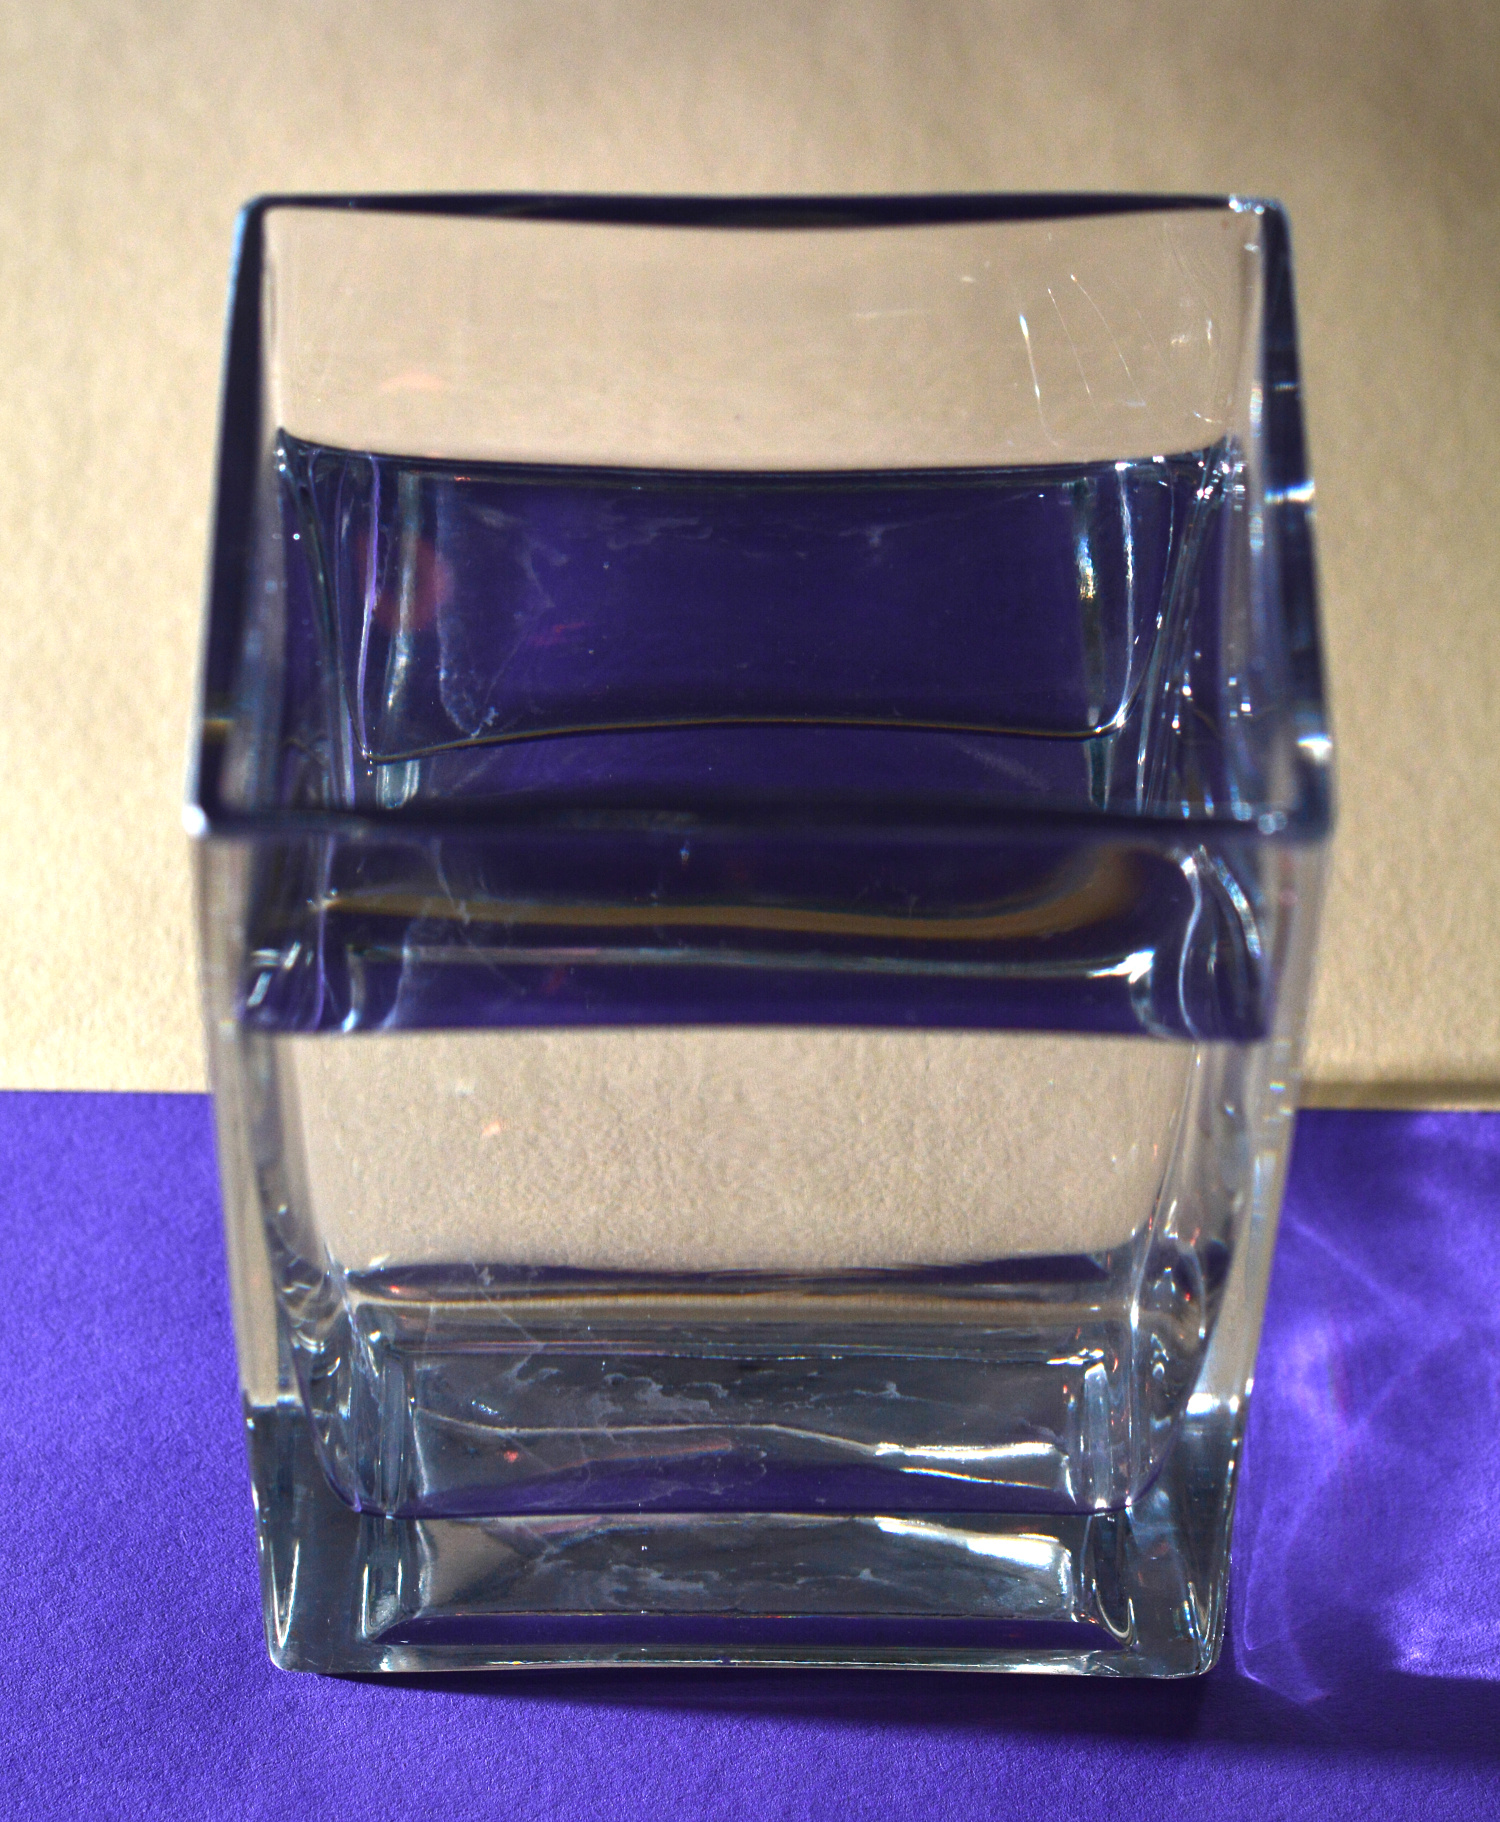
\includegraphics[width=5.5truecm]{slike/04_TIRF1.jpg}\qquad \qquad
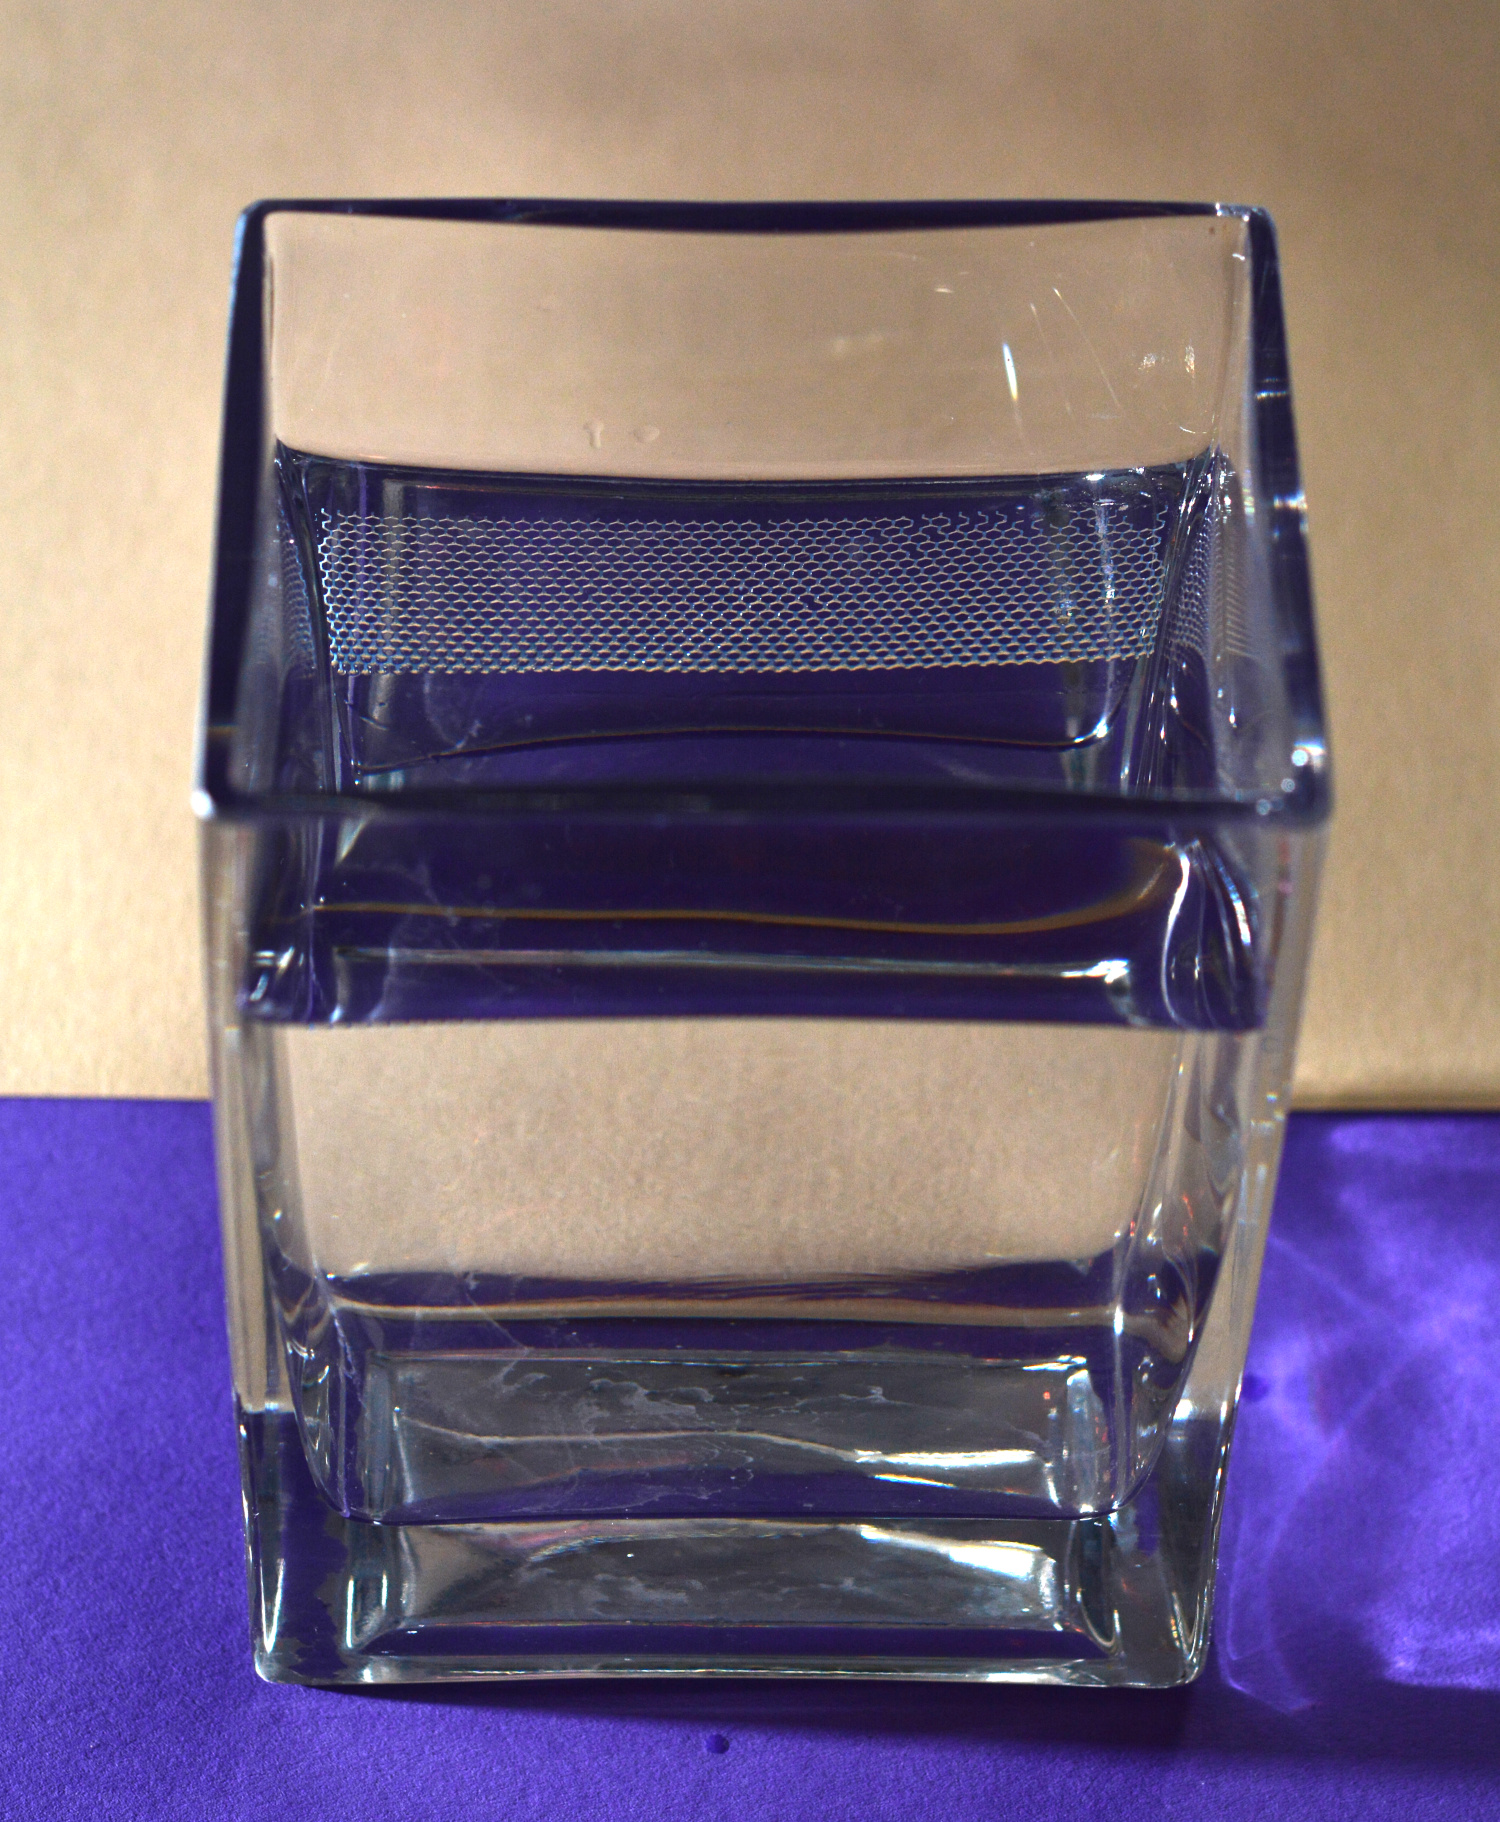
\includegraphics[width=5.5truecm]{slike/04_TIRF2.jpg}
\caption{Svetloba se ob prehodu iz vode v zrak na zadnji steni steklene vaze 
totalno odbije, zato tam vidimo vijolično dno (levo). Ko ob zadnjo steno prislonimo
navlaženo mrežasto tkanino, na mestih stika totalnega odboja ni več in svetloba prehaja
skozi mejo kljub vpadnemu kotu, večjemu od mejnega kota totalnega odboja (desno).
Podobno delujejo čitalci prstnih odtisov.}
\label{fig:04_FTIRfoto}

\end{figure}
\begin{remark}
Pri totalnem odboju se zgodi še en zanimiv pojav, ki ga imenujemo Goose--H\"anchenin pojav 
po nemških fizikih Hermannu Fritzu Gustavu Goosu (1883--1968) in Hildi H\"anchen (1919--2013).
Ko se linearno polarizirana svetloba totalno odbije, odbita svetloba ne izhaja iz 
povsem iste točke, kot nanjo vpada. Videti je, kot da se svetloba odbije od neke 
navidezne ravnine, ki leži v snovi z manjšim lomnim količnikom. 
Oddaljenost te navidezne odbojne ravnine je kar enaka vdorni globini, 
zato je vzporeden premik enak: $L = 2d_v\,\tan(\alpha)$.

Pojava z opisom poti enega žarka svetlobe ne moremo pojasniti, temveč moramo
obravnavati snop svetlobe, sestavljen iz več žarkov. Žarki vpadajo na mejo pod rahlo
različnimi vpadnimi koti, zato imajo po odboju rahlo različno fazo. Skupni 
učinek faznih zakasnitev je tak, kot bi se žarek navidezno vzdolžno premaknil. 
\begin{figure}[ht]
\centering
\def\svgwidth{70truemm} 
\input{slike/04_Goos.pdf_tex}
\caption{Goos-H\"anchenin pojav pri totalnem odboju: totalno odbita svetloba izhaja iz druge točke, 
kot vpada na mejo snovi vpada svetloba. Videti je, kot da se odbije od navidezne ravnine.}
\label{fig:04_Goos}
\vglue-5truemm\end{figure}
\end{remark}

\section{Faza pri totalnem odboju}
Poglejmo še, kaj se zgodi s fazo valovanja pri odboju na meji dveh snovi. 
Pri navadnem odboju, pri katerem sta koeficienta
amplitudne odbojnosti za obe polarizaciji realna, ni težav. 
Pogledati moramo samo predznak $r$ v Fresnelovih enačbah (enačbi~\ref{eq:TEr} 
in \ref{eq:TMr}). Pri odboju na 
optično gostejšem sredstvu se faza TE polariziranega valovanja 
spremeni za $\pi$, faza TM polariziranega
valovanja pa pri Brewstrovem kotu preskoči s $\pi$ na 0. 
Pri vpadu na optično redkejšo snov se faza
TE polarizacije ohranja, faza TM polarizacije pa pri 
Brewstrovem kotu preskoči z 0 na $\pi$.  

Zanimivejša je faza pri totalnem odboju. V prejšnjem razdelku smo spoznali atenuacijski koeficient
$\varkappa$, ki je močno odvisen od vpadnega kota in tudi od polarizacije valovanja (enačbi~\ref{eq:kappatot} 
in \ref{eq:kappatottm}):
\beq
\varkappa_{\mathrm{TE}}= k_0 n_2 \sqrt{\left(\frac{\sin \alpha}{\sin \alpha_m}\right)^2-1} 
\qquad \mathrm{in}\qquad
\varkappa_{\mathrm{TM}}= k_0 n_1 \sqrt{\left(\frac{\sin \alpha}{\sin \alpha_m}\right)^2-1}.
\label{eq:04_83}
\eeq
Valovanje v obliki evanescentnega vala vdira v snov z manjšim lomnim količnikom, zato
pri oboju doživi fazni zamik. Ker je fazni zamik neposredno povezan z atenuacijskim
koeficientom oziroma vdorno globino, je odvisen od vpadnega kota $\alpha$ in polarizacije svetlobe. 


Izračunajmo najprej fazo za TE polarizirano valovanje. Izhajamo iz amplitudne odbojnosti (enačba~\ref{eq:04_61})
in kompleksni števili v števcu in imenovalcu zapišemo v polarni obliki:
\beq
r_\mathrm{TE} = \frac{n_1 \cos \alpha - i n_2 \kappa}{n_1 \cos \alpha + i n_2 \kappa} = 
\frac{\sqrt{n_1^2\cos^2 \alpha + n_2^2 \kappa^2}\,e^{-i\delta_\mathrm{TE}/2}}{\sqrt{n_1^2\cos^2 \alpha + n_2^2 \kappa^2}\,e^{+i\delta_\mathrm{TE}/2}}
= e^{-i\delta_\mathrm{TE}},
\label{eq:04_84}
\eeq
pri čemer je:
\beq
\delta_\mathrm{TE} = 2\arctan\frac{n_2\kappa}{n_1 \cos \alpha} = 2\arctan\frac{n_2 \sqrt{\left(\frac{\sin \alpha}{\sin \alpha_m}\right)^2-1}}{n_1 \cos \alpha} = 
2\arctan\frac{\sqrt{n_1^2\sin^2 \alpha-n_2^2}}{n_1 \cos \alpha}.
\label{eq:04_85}
\eeq
Fazni zamik totalno odbitega valovanja je torej odvisen od vpadnega kota $\alpha$. 
Pri $\alpha = \alpha_m$ je vrednost $\delta=0$, pri vpadnem kotu $\alpha \to 90\si{\degree}$ pa je
fazni zamik odbitega valovanja $\delta = \pi$. Vmesna odvisnost je prikazana na sliki~\ref{fig:04_faza}.
\begin{figure}[ht]
\centering
\def\svgwidth{80truemm} 
\input{slike/04_faza.pdf_tex}
\caption{Fazna zamika totalno odbite svetlobe in 
njuna razlika $\Delta$ v odvisnosti od vpadnega kota $\alpha$ za obe polarizaciji.}
\label{fig:04_faza}
\end{figure}

Podoben rezultat dobimo tudi za TM polarizirano valovanje, le da sta lomna količnika $n_1$ in $n_2$
zamenjana. Tako velja:
\beq
\delta_\mathrm{TM}= 2\arctan\frac{n_1\kappa}{n_2 \cos \alpha} = 2\arctan\frac{n_1 \sqrt{\left(\frac{\sin \alpha}{\sin \alpha_m}\right)^2-1}}{n_2 \cos \alpha}.
\label{eq:04_86}
\eeq
Ker je predpogoj za totalni odboj $n_1 > n_2$, so vrednosti faznega zamika za 
TM polarizacijo vedno večje od faznega zamika za TE polarizirano
valovanje. 

Velja namreč:
\beq
\tan \frac{\delta_\mathrm{TM}}{2} = \left(\frac{n_1}{n_2}\right)^2 \tan \frac{\delta_\mathrm{TE}}{2}
\label{eq:04_87}
\eeq
in posledično:
\beq
\Delta = \delta_\mathrm{TM}-\delta_\mathrm{TE} \ge 0.
\label{eq:04_88}
\eeq
Če je razmerje lomnih količnikov dovolj veliko, lahko razlika faznih zamikov doseže vrednost, ki je
večja od $\pi/4$. To se, na primer, lahko zgodi pri totalnem odboju na meji med steklom in zrakom. 
Kadar je fazna razlika med obema polarizacijama pri odboju tako velika, lahko  z dvema zaporednima
totalnima odbojema pri nekem vpadnem kotu $\alpha$
dosežemo fazni zamik med TE in TM polariziranim valovanjem, ki je enak $\pi/2$. 
Optični element, v katerem pride do dveh zaporednih totalnih odbojev, torej lahko deluje kot ploščica
$\lambda/4$. S štirimi totalnimi odboji dobimo fazni zamik $\pi$ in učinek ploščice $\lambda/2$. Tovrstni optični elementi se imenujejo Fresnelovi rombi. 
Njihova glavna prednost je v tem, da delujejo neodvisno od 
valovne dolžine $\lambda$, saj ta ne nastopa eksplicitno v izrazu za $\Delta$. Popravke 
višjega reda, na primer odvisnost lomnega količnika od valovne dolžine, tukaj zanemarimo.
\begin{figure}[ht]
\centering
\def\svgwidth{70truemm} 
\input{slike/04_Fresneltot.pdf_tex}
\caption{V Fresnelovem rombu se vpadna svetloba dvakrat totalno odbije, pri čemer
se med polarizacijama pojavi zamik $\pi/2$. Iz vpadne linearne polarizacije pod kotom 
$45\si{\degree}$ nastane krožno polarizirano valovanje in Fresnelov romb deluje 
kot ploščica $\lambda/4$. Romb je narejen tako, da je iskan fazni 
zamik dosežen pri pravokotnem vpadu.}
\label{fig:04_Fresneltot}
\end{figure}

\section{Odboj na kovinah}
\label{section:410}
Zanimivo vprašanje je, kako se Fresnelove enačbe spremenijo, če je snov, 
na katero svetloba vpada, prevodna. V tem primeru
vemo, da polje pojema z globino zaradi notranjih električnih tokov. 
Po analogiji s totalnim odbojem, pri katerem evanescentno polje prav tako
pojema z globino, pričakujemo, da bo odbojnost na meji velika. 

Ker je zaradi meje simetrija prostora zlomljena le v smeri osi $z$, polje
lahko pojema le z globino, to je s koordinato $z$. 
Omejimo se zaenkrat na TE polarizirano valovanje, ki 
ga v prevodni snovi zapišemo kot:
\beq
\mathbf{E}_2 = \mathbf{e}_y E_{0t} e^{i(k_z+i\varkappa)z} e^{ik_xx-i\omega t}.
\label{eq:04_89}
\eeq
Komponenta valovnega vektorja, ki je vzporedna z mejno ploskvijo, je zaradi
robnih pogojev enaka na obeh straneh meje. Zapišemo jo kot: $k_x = k_0 n_1 \sin \alpha$. 

Za opis valovanja v prevodni snovi moramo namesto valovne enačbe uporabiti telegrafsko enačbo 
(enačba~\ref{eq:telegrafska}). Kompleksno valovno število izrazimo s 
kompleksnim lomnim količnikom $\mathcal{N}$ (enačba~\ref{eq:nkompleks2}):
\beq
|\tilde{\mathbf{k}}|^2 = k_x^2 + (k_z+i\varkappa)^2 = k_0^2 \mathcal{N}^2  = 
k_0^2 \left(\varepsilon_2 + \frac{i\sigma_2}{\varepsilon_0 \omega}\right)\!\!,
\label{eq:04_90}
\eeq
pri čemer $\epsilon_2$ in $\sigma_2$ označujeta dielektričnost in električno
prevodnost druge (prevodne) snovi. Iz tega sledi:
\beq
\frac{k_x^2+k_z^2 - \varkappa^2}{k_0^2} + \frac{2 i \varkappa k_z}{k_0^2} = \varepsilon_2 + 
\frac{i \sigma_2}{\varepsilon_0 \omega}.
\label{eq:04_91}
\eeq
Parametra $k_z$ in $\varkappa$ izračunamo iz enačbe:
\beq
k_z^2 - \varkappa^2+ 2 i \varkappa k_z= k_0^2 \varepsilon_2 - k_x^2 + i\frac{k_0^2\sigma_2}{\varepsilon_0 \omega}.
\label{eq:04_92}
\eeq
Postopamo podobno, kot pri izračunu kompleksnega lomnega količnika, in dobimo:
\beq
k_z^2 = \frac{1}{2}\left(\sqrt{\left(k_0^2\varepsilon_2-k_x^2\right)^2 + \left(\frac{\sigma_2 k_0^2}{\varepsilon_0 \omega}\right)^2}
+ k_0^2\varepsilon_2-k_x^2 \right)
\label{eq:04_93}
\eeq
in 
\beq
\varkappa^2 = \frac{1}{2}\left(\sqrt{\left(k_0^2\varepsilon_2-k_x^2\right)^2 + \left(\frac{\sigma_2 k_0^2}{\varepsilon_0 \omega}\right)^2}
- k_0^2\varepsilon_2+k_x^2\right)\!\!.
\label{eq:04_94}
\eeq
Celotno komponento valovnega vektorja v smeri $z$ v prevodni snovi potem zapišemo kot vsoto 
realnega in imaginarnega dela:
\beq
\tilde{k}_z = k_z + i \varkappa.
\label{eq:04_95}
\eeq
Zapišimo robne pogoje, po katerih se ohranjata tangentni komponenti jakosti
električnega in magnetnega polja (enačbi~\ref{eq:RPE} in \ref{eq:RPH}).Prva enačba
je preprosta:
\beq
E_{0i} + E_{0r} = E_{0t}.
\label{eq:04_97}
\eeq
Drugo enačbo dobimo z upoštevanjem Faradayevega zakona (enačba~\ref{eq:Maxwell2}).
Izvrednotimo časovni odvod magnetnega polja in dobimo zvezo: $\nabla \times \mathbf{E}
= i \omega \mu_0 \mathbf{H}$. Na meji se ohranja tangentna komponenta $H_x$ (glej
sliko~\ref{fig:04_tetm}), zato
se na meji ohranja odvod jakosti električnega polja $dE/dz$:
\beq
-ik_{1z}E_{0i} + ik_{1z}E_{0r}= -(ik_{2z}+\varkappa)E_{0t}.
\label{eq:04_98}
\eeq
Eliminiramo neznanko $E_{0t}$ in izračunamo amplitudno odbojnost:
\boxeq{eq:Kovinar}{
r = \frac{E_{0r}}{E_{0i}} = \frac{k_{1z}-k_{2z}-i \varkappa}{k_{1z}+k_{2z}+i\varkappa}.
}
Tak rezultat je pričakovan. Spomnimo se amplitudne odbojnosti za navadni neprevodni primer
(enačba~\ref{eq:TEr}):
\beq
r = \frac{n_1 \cos \alpha - n_2 \cos \beta}{n_1 \cos \alpha + n_2 \cos \beta} = 
\frac{k_0 n_1 \cos \alpha - k_0 n_2 \cos \beta}{k_0 n_1 \cos \alpha + k_0 n_2 \cos \beta} = 
\frac{k_{1z}-k_{2z}}{k_{1z}+k_{2z}}.
\label{eq:04_96}
\eeq
V primeru prevodne snovi je izraz povsem enak, le da namesto
realne vrednosti komponente valovnega vektorja v drugi snovi $k_{2z}$ 
upoštevamo kompleksno vrednost komponente $\tilde{k}_z = k_{2z}+ i\varkappa$. Realni del 
je tako enak kot v neprevodnih snoveh, imaginarni del pa je enak kot pri totalnem odboju
na meji dveh neprevodnih snovi (enačba~\ref{eq:04_54}). 
Temu ustrezno lahko rezultat razumemo kot neko vmesno rešitev, ki delno spominja
na navadni odboj, vendar ima večjo odbojnost. Kovine zato dobro odbijajo svetlobo
in se ``bleščijo''. 
 
Zapišimo amplitudno odbojnost za TE polarizirano valovanje še drugače:
\boxeq{eq:04_99}{
r_\mathrm{TE} = \frac{n_1 \cos \alpha - \mathcal{N}_2 \cos
\beta}{n_1 \cos \alpha + \mathcal{N}_2 \cos \beta}.
}
Pri tem je $\cos \beta$ kompleksno število, določeno formalno 
z lomnim zakonom $n_1 \sin \alpha = \mathcal{N}_2 \sin \beta$.
Sklepamo, da po analogiji amplitudno odbojnost za TM polarizirano valovanje zapišemo kot: 
\boxeq{eq:04_100}{
r_\mathrm{TM} = \frac{\mathcal{N}_2 \cos \alpha - n_1
\cos \beta}{\mathcal{N}_2 \cos \alpha + n_1 \cos \beta}.
}


Odbojnost $\mathcal{R}$, ki jo izračunamo kot:
\beq
\mathcal{R} = |r|^2,
\label{eq:04_100a}
\eeq
je prikazana na sliki~\ref{fig:04_kovina}. Odbojnost za TE polarizacijo
homogeno narašča z naraščajočim vpadnim kotom 
od neke začetne vrednosti pri pravokotnem vpadu do 1. 
Intenziteta TM polarizacije na prevodnih snoveh 
nikoli ne pade na nič, se pa pri določenih kotih občutno
zmanjša (analog Brewsterjevem kotu pri odboju na neprevodnih snoveh).
\begin{figure}[ht]
\centering
\def\svgwidth{70truemm} 
\input{slike/04_kovinaMo.pdf_tex}
\caption{Odbojnost na prevodni snovi v odvisnosti od vpadnega kota za TE in TM polarizirano
valovanje. Primer je narisan za molibden z $n'=3,70$ in $n''=3,55$.}
\label{fig:04_kovina}
\end{figure}

Račun odboja na kovini je razmeroma zapleten. Preprost je le v primeru pravokotnega vpada, 
ko sta $\alpha = \beta = 0$. Takrat dobimo za amplitudno odbojnost:
\beq
r = \frac{n_1 - \mathcal{N}}{n_1 + \mathcal{N}} = \frac{n_1 -n_2' -in_2''}{n_1 +n_2' +in_2''},
\label{eq:04_101}
\eeq
pri čemer $n_2'$ označuje realni in $n_2''$ imaginarni del kompleksnega lomnega količnika.
Izračunamo še odbojnost:
\beq
\mathcal{R} = |r|^2 = \frac{(n_1 -n_2')^2 +n_2''^2}{(n_1 +n_2')^2 +n_2''^2}.
\label{eq:04_102}
\eeq
Kadar je realni del $n'$ lomnega količnika zelo majhen, lahko izraz še poenostavimo 
in dobimo:
\beq
\mathcal{R} = \frac{n_1^2 +n_2''^2}{n_1^2 +n_2''^2} = 1.
\label{eq:04_103}
\eeq
Snovi z majhnim realnim delom lomnega količnika $n'$ torej vso vpadno 
svetlobo odbijejo. Primera takih kovin sta srebro ($n'=0,15$ in $n''=3,9$)
in aluminij ($n'=1,3$ in $n''=7,3$). Obe kovini zato uporabljamo za izdelavo
zrcal.
\begin{figure}[ht]
\centering

\includegraphics[width=6truecm]{slike/04_photos_kovina.jpg}
\caption{Gladka površina dobro prevodnih kovin odbija praktično 
vso vpadno svetlobo, zato jih uporabljamo za izdelavo zrcal. Kuhinjska aluminijasta
folija na sliki ni povsem gladka, zato je zrcalna slika popačena.}
\label{fig:04_KovinaFoto}
\end{figure}
